\documentclass[a4paper,english,twoside,openright,11pt]{book}
\usepackage{cmap} % makes PDF searchable
\usepackage{babel}
\usepackage{tabulary}
%\usepackage[latin9]{inputenc}
\usepackage[latin1]{inputenc}
\usepackage{lmodern} % Latin Modern font
\usepackage[T1]{fontenc}
\usepackage{textcomp} % needed for fontenc
%\usepackage{styles/extref}
\usepackage[bookmarksnumbered,final]{styles/easyoutput}
\usepackage{url}
\usepackage[final]{listings}
	\lstset{numbers=left,breaklines}
\usepackage{acronym}
\usepackage{makeidx}
	\makeindex
%\usepackage[square]{natbib}
\usepackage[binding=0.8cm]{styles/layaureo} % better handling of A4 format
\usepackage{tocbibind} 
\usepackage[labelfont=bf]{caption}[2004/07/16] % format of captions
\usepackage{subfig}
% tables
\usepackage{booktabs}
\usepackage{tabulary}
% citations at the beginning of each chapter
\usepackage{epigraph}
	\setlength{\epigraphwidth}{.59\textwidth}
	\renewcommand{\epigraphsize}{\small}
	\renewcommand{\epigraphflush}{flushleft}
\usepackage{styles/reallyblank} % insert empty page at the beginning of a chapter with empty headings
% the following is for thesis in Italian language; adapt it for English ones
\usepackage{sistyle}
\AddToSIstyle{English}{
   \SIdecimalsign{,}
   \SIthousandsep{\,}
   \SIproductsign{\cdot}
   \SIunitsep{\,}
   \SIunitspace{\,}
   \SIunitdot{\cdot}
   \SIobeyboldfalse
   \SIgroupfourfalse}
\SIstyle{English}
\usepackage{verbatim}

% used to use the footnote inside a figure's caption
\usepackage{afterpage}

\usepackage{gensymb}
\usepackage{wasysym}
\usepackage{amsfonts}
\usepackage{graphicx}

\newcommand{\dspic}{dsPIC$^{\text{\textregistered}}$ DSC}
\newcommand{\dcbus}{DC-BUS\texttrademark }

% listings for source code
\usepackage{listings}

\lstset{language=[ANSI]C,
numbersep=5pt,
numberstyle=\tiny,
numbers=none,
basicstyle=\linespread{0.8}\footnotesize
}

\usepackage{csquotes}
\usepackage{cleveref}

% toOl: set linespread to 1 in the verbatim environment
\makeatletter
\def\verbatim@font{\linespread{1}\normalfont\ttfamily}
\makeatother

\title{This is the title of my thesis}
\author{John Doe}
\date{Academic Year 2007/2008}
\subject{Master Thesis in computer Engineering at University of Pavia}

\renewcommand{\baselinestretch}{1.3}

\begin{document}
\frenchspacing
\frontmatter

%-------------------------------------------------------------------
% Frontmatter
%-------------------------------------------------------------------

\begin{titlepage}

\thispagestyle{empty}

\begin{center}
\vskip 1cm

\includegraphics[width=4cm]{figs/logo-unipv-bw}
\vskip 0.5cm

\LARGE
	\textbf{University of Pavia}\\
	\textbf{Faculty of Engineering}\\
	\textbf{Department of Electrical, Computer and Biomedical Engineering}

\vskip 0.5cm

\Large
	\printgraduation
	
\vskip 1.5cm

\Huge
	\textbf{\printtitle}

\vskip 1.5cm
	
\Large

\begin{minipage}[t]{7cm}
	Supervisor:\\
	\printsupervisor \\
\end{minipage}

\hfill

\begin{minipage}[t]{5cm}
	Candidate:\\
	\printauthor\\
	%Matricola: 348374/46
\end{minipage}

\vskip 1.5cm

	Academic Year \printacademicyear

\end{center}

\vfill
\eject
\end{titlepage}


\thispagestyle{empty}
\mbox{}
\newpage

%
\begin{flushright}
\thispagestyle{empty}
\null\vspace*{\stretch{1}}
{\it Here you can write whatever you want

\vspace{10pt}
and here too.
}
\vspace{\stretch{2}}\null
\end{flushright}
%
\thispagestyle{empty}
\mbox{}
\newpage
%
\chapter*{Acknowledgments}

Some acknowledgments to family, friends, supervisors, etc.

\thispagestyle{empty}
\mbox{}
\newpage

%-------------------------------------------------------------------
% Indexes
%-------------------------------------------------------------------
\tableofcontents
\listoffigures
\listoftables


\mainmatter
%-------------------------------------------------------------------
\chapter*{Acronyms}
%-------------------------------------------------------------------

\begin{acronym}
\acro{LED}{Light Emitting Diode}
\acro{UNIPV}{University of Pavia}
\acro{Robolab}{Robotics Laboratory}
\end{acronym}

%-------------------------------------------------------------------
\chapter{Introduction}
\label{c:intro}
%-------------------------------------------------------------------

\section{Background}
Under the name "Depth Estimation" (DE) a lot of techniques appear, but there is no formal definition that considers them all.
I would define DE as the study of algorithms that process one or more images of a scene and output information about its geometry.
There exist many approaches to do this as well as many problem settings.
The setting of this thesis is \textit{Single Image Depth Estimation}, also called \textit{Monocular Depth Estimation}.
It refers to a depth estimation problem based on only one image of the scene.

As it is often the case in computer science, there is no such thing as the best algorithm for solving a given problem, rather there are several and each with its own advantages and disadvantages, some more successful than others.
Brilliant minds have contributed to this field and in this chapter I will present some of their ideas.


This is not mathematics, there aren't rigid formal definitions and formulas and symbols don't follow strict rules.
Notation serves clarity.
The treatment is informal though mathematically informed.


\textbf{Images} are what we want to extract geometry informations from.
Images are represented as two (gray images) or three (color images) dimensional arrays of limited positive numbers.
Color images can be in turn represented in different color spaces.
Images can be resized through sampling and interpolation.
I will usually refer to an image using the letters $I$ and $J$.
A pixel is a location on an image and is indexed using a pair of numbers $(i, j)$, sometimes written $ij$ or it can be indexed using a single letter like $i$ or $p$.
For gray images the value of an image in a certain pixel is a single number, while for color images it is a triad of numbers corresponding to some color space representation, usually RGB.
$I_{ij}$ denotes such values.
$ij$ can be a non-integer pair of numbers, in such a case $I_{ij}$ will still make sense and a \textit{differentiable} sampling procedure is implied(usually the one used in \cite{STN}).


\textbf{Depth maps} are often the output of depth estimation algorithms.
A depth map is an image in which every pixel value represents a depth measure, meaning the distance from the image plane or, equivalently, the $Z$ coordinate of a point $\mathbf{x} = (X, Y, Z)$ in space, where $X$ and $Y$ corresponds to the image plane coordinates.
Since only points in front of the camera are considered, $Z$ values are always strictly positive.
I will usually refer to a depth map using the symbol $\mathbf{Z}$.
$\mathbf{Z}$ can be a \textit{metric} depth map, meaning each pixel value represents a spatial distance expressed in absolute physical units (e.g. meters), or it can be a \textit{relative} depth map and only used for relative depth comparisons of pairs of pixel (e.g. which pixel is closer or farther).
An important kind of a relative depth map is an \textit{affine} depth map, that is a depth map equals to the metric depth map of the scene up to an affine transformation: $\mathbf{Z}_{metric} = s \, \mathbf{Z}_{affine} + t$ for some $s, t$.

Following an image formation model, in both images and depth maps every pixel value is determined by some property of a 3D scene location which I will denote as $\mathbf{x}$, be it distance, reflectance, color, texture, ...
The camera acquiring the image has \textit{intrinsic} parameters describing its acquisition geomtry and \textit{extrinsic} ones refering to its position in space.
Projective geometry is used for expressing camera and image geometry \cite{multiview}.
I won't go into its details, suffice it to say that by knowing these parameters one is able to \textit{project} a 3D location $\mathbf{x}$ to the image plane and by knowing the distance(depth) $Z$ of such a point and its location $(i,j)$ in the image plane also the reverse is doable, namely \textit{backprojecting} the pixel to a 3D location.


\textbf{Disparity maps} are a concept related to the so called \textit{stereo} or \textit{binocular} depth estimation where scene geometry must be infered from two images.
Disparity maps will be indicated by $\mathbf{D}$. In order to understand what they are, assume there is an object in the scene at $\mathbf{x}$ and two identical cameras simulteneously take a picture from slightly different angles.
The object location in the first image $(i_{1}, j_{1})$ will be different from its location in the second image $(i_{2}, j_{2}) $(imagine overlapping the two images).
A displacement $d = (i_{2} - i_{1}, j_{2} - j_{1})$ is thus obtained.
By knowing extrinsic and intrinsic parameters of the two cameras, depth $Z$ from the first camera corresponding to $(i_{1}, j_{1})$ can be computed by means of such displacement.

Thus, for every pixel $(i, j)$ of the first image, by backprojecting it in 3D space and then projecting it on the second image a displacement $\mathbf{D}(i,j)$ can be computed.
The mapping from pixel to displacement is called a disparity map, in this example we computed the disparity map of the first image w.r.t. the second.
Analogously a disparity map can be computed for the second image w.r.t. the first.
There exist pixels for which this procedure fails either because the projection of $\mathbf{x}$ onto the other image ends up out-of-view or because $\mathbf{x}$ is occluded from the other perspective and does not contribute to image formation.
Hence disparity maps can have "holes" in which they are not defined.

In the very simple setting of identical cameras put side to side (mounted on a \textit{stereo-rig}) pointing at parallel directions, the disparity $d$ is a one dimensional displacement and is represented by a single real number.
This will be the case from here on. The obtained image pair is called \textit{rectified}.


The problem of depth estimation is to design an algorithm that can reconstruct the geometry of a scene from $N$ images of it.
A function $f$ is required such that $f(I_{1}, I_{2}, ..., I_{N})$ represents such geometry, usually as a depth map $\mathbf{Z}$ or disparity map $\mathbf{D}$, but other representations exist in particular when $N > 2$, i.e. \textit{multi-view} case.
There exist surveys treating the problem for $N \geq 2$ \cite{correspondance, stereo}, but the focus of this thesis is the case $N = 1$, namely \textit{monocular} or \textit{single image} depth estimation.


In the \textbf{deep learning} approach $f$ is called a $model$ and has \textit{trainable} parameters which must be tuned minimizing what is called a \textit{loss function} $\mathcal{L}$, that is: a quantity expressing some undesired property that $f$ mustn't satisfy.
For it to be minimized during a first phase called \textit{training}, differentiability of $\mathcal{L}$ in the trainable parameters is required.
This implies that $f$ itself should be differentiable in them.
Algorithms based on gradient descent are employed for optimization.
$\mathcal{L}$ is often expressed as a sum of other loss functions and so called \textit{regularization} terms which serve the overall training procedure, favouring the \textit{generalization} of the model.
A model is said to generalize well when its predictions are reliable on new input data, i.e. not seen during training.
This whole procedure is only possibile if a \textit{dataset} is given, that is a collection of data statistically defining the desired behaviour of $f$.
It can be a set of input-output pairs, e.g. images and associated depth maps, or a more general data collection, e.g. video footage.
The desired output of the model in response to a certain input is called \textit{ground-truth}.

\textit{Testing} follows training.
During the testing phase the model generalization capability is evaluated on new data using \textit{metrics} $\mathcal{M}$ which quantitatively express the \textit{error} the model is committing (like loss functions do, hence the smaller the better) or its \textit{accuracy} (the greater the better).
In order to test a model a dataset containing ground-truth data is necessary so that the desired behaviour can be quantitatively compared with the actual behaviour.
The output of a model is often called a \textit{prediction}, so metrics $\mathcal{M}$ are functions of both predictions and ground truth data.


\textit{Statistical learning} is the predecessor of deep learning and it shares with it the same theoretical foundations, but it proved to be less effective.
Deep learning efficacy is mainly due to its scalability in training, meaning that very large datasets can be used and the resulting optimization problem is computationally feasible for the existing hardware, although the costs are not always affordable.

%During testing time all monocular depth estimation models are able to infer depth from a single image, however during training the kind of data they require can vary from tecnique to tecnique.
%Chapter 2 treats these differences. In its "Supervised" section models trained on ground-truth data are presented, while in the "Self Supervised" one ground-truth is not necessary and data can be video footage or stereo pairs.
%Instead in "Classic" techniques not necessarily based on deep learning(and hence on datasets) are reviewed.
%
%In this chapter some of the ideas developed for solving monocular depth estimation are reviewed.
%The "Classic" section is about works that don't use what we'd call deep learning.
%"Supervised" , "Self Supervised" and in particular "SOTA" are solely about deep learning techniques.
%Datasets and metrics details are encapsulated in the "Datasets" and "Metrics" sections.
%
%
%I won't spend too much time on neural network architectures and in particular on explaining numerical details and experiments.
%If a method appears in this chapter it means that it was successful in its intent.
%The scale of efficacy is Classic $<$ Self Supervised $<$ Supervised $<$ SOTA.


%-------------------------------------------------------------------
\chapter{State of the art}
\label{c:sota}
%-------------------------------------------------------------------

\epigraph{\enquote{The wireless telegraph is not difficult to understand. The ordinary telegraph is like a very long cat. You pull the tail in New York, and it meows in Los Angeles. The wireless is the same, only without the cat.}}{\emph{Albert Einstein}}

This chapter provides an overview of the state of the art.

%\section{Background}
Under the name "Depth Estimation" a lot of techniques appear, but there is no formal definition that considers them all.
I would define "Depth Estimation" as the study of algorithms that process one or more images of a scene and output information about its geometry.
There exist many approaches to do this as well as many problem settings.
The setting of this thesis is \textit{Single Image Depth Estimation}, also called \textit{Monocular Depth Estimation}.
It refers to a depth estimation problem based on only one image of the scene.

As it is often the case in computer science, there is no such thing as the best algorithm for solving a given problem, rather there are several and each with its own advantages and disadvantages, some more successful than others.
Brilliant minds have contributed to this field and in this chapter I will present some of their ideas.


This is not mathematics, there aren't rigid formal definitions and formulas and symbols don't follow strict rules.
Notation serves clarity.
The treatment is informal though mathematically informed.


\textbf{Images} are what we want to extract geometry informations from.
Images are represented as two (gray images) or three (color images) dimensional arrays of limited positive numbers.
Color images can be in turn represented in different color spaces.
Images can be resized through sampling and interpolation.
I will usually refer to an image using the letters $I$ and $J$.
A pixel is a location on an image and is indexed using a pair of numbers $(i, j)$, sometimes written $ij$ or it can be indexed using a single letter like $i$ or $p$.
For gray images the value of an image in a certain pixel is a single number, while for color images it is a triad of numbers corresponding to some color space representation, usually RGB.
$I_{ij}$ denotes such values.
$ij$ can be a non-integer pair of numbers, in such a case $I_{ij}$ will still make sense and a \textit{differentiable} sampling procedure is implied(usually the one used in \cite{STN}).


\textbf{Depth maps} are often the output of depth estimation algorithms.
A depth map is an image in which every pixel value represents a depth measure, meaning the distance from the image plane or, equivalently, the $Z$ coordinate of a point $\mathbf{x} = (X, Y, Z)$ in space, where $X$ and $Y$ corresponds to the image plane coordinates.
Since only points in front of the camera are considered, $Z$ values are always strictly positive.
I will usually refer to a depth map using the symbol $\mathbf{Z}$.
$\mathbf{Z}$ can be a \textit{metric} depth map, meaning each pixel value represents a spatial distance expressed in absolute physical units (e.g. meters), or it can be a \textit{relative} depth map and only used for relative depth comparisons of pairs of pixel (e.g. which pixel is closer or farther).
An important kind of a relative depth map is an \textit{affine} depth map, that is a depth map equals to the metric depth map of the scene up to an affine transformation: $\mathbf{Z}_{metric} = s \, \mathbf{Z}_{affine} + t$ for some $s, t$.

Following an image formation model, in both images and depth maps every pixel value is determined by some property of a 3D scene location which I will denote as $\mathbf{x}$, be it distance, reflectance, color, texture, ...
The camera acquiring the image has \textit{intrinsic} parameters describing its acquisition geomtry and \textit{extrinsic} ones refering to its position in space.
Projective geometry is used for expressing camera and image geometry \cite{multiview}.
I won't go into its details, suffice it to say that by knowing these parameters one is able to \textit{project} a 3D location $\mathbf{x}$ to the image plane and by knowing the distance(depth) $Z$ of such a point and its location $(i,j)$ in the image plane also the reverse is doable, namely \textit{backprojecting} the pixel to a 3D location.


\textbf{Disparity maps} are a concept related to the so called \textit{stereo} or \textit{binocular} depth estimation where scene geometry must be infered from two images.
Disparity maps will be indicated by $\mathbf{D}$. In order to understand what they are, assume there is an object in the scene at $\mathbf{x}$ and two identical cameras simulteneously take a picture from slightly different angles.
The object location in the first image $(i_{1}, j_{1})$ will be different from its location in the second image $(i_{2}, j_{2}) $(imagine overlapping the two images).
A displacement $d = (i_{2} - i_{1}, j_{2} - j_{1})$ is thus obtained.
By knowing extrinsic and intrinsic parameters of the two cameras, depth $Z$ from the first camera corresponding to $(i_{1}, j_{1})$ can be computed by means of such displacement.

Thus, for every pixel $(i, j)$ of the first image, by backprojecting it in 3D space and then projecting it on the second image a displacement $\mathbf{D}(i,j)$ can be computed.
The mapping from pixel to displacement is called a disparity map, in this example we computed the disparity map of the first image w.r.t. the second.
Analogously a disparity map can be computed for the second image w.r.t. the first.
There exist pixels for which this procedure fails either because the projection of $\mathbf{x}$ onto the other image ends up out-of-view or because $\mathbf{x}$ is occluded from the other perspective and does not contribute to image formation.
Hence disparity maps can have "holes" in which they are not defined.

In the very simple setting of identical cameras put side to side (mounted on a \textit{stereo-rig}) pointing at parallel directions, the disparity $d$ is a one dimensional displacement and is represented by a single real number.
This will be the case from here on. The obtained image pair is called \textit{rectified}.


The problem of depth estimation is to design an algorithm that can reconstruct the geometry of a scene from $N$ images of it.
A function $f$ is required such that $f(I_{1}, I_{2}, ..., I_{N})$ represents such geometry, usually as a depth map $\mathbf{Z}$ or disparity map $\mathbf{D}$, but other representations exist in particular when $N > 2$, i.e. \textit{multi-view} case.
There exist surveys treating the problem for $N \geq 2$ \cite{correspondance, stereo}, but the focus of this thesis is the case $N = 1$, namely \textit{monocular} or \textit{single image} depth estimation.


In the \textbf{deep learning} approach $f$ is called a $model$ and has \textit{trainable} parameters which must be tuned minimizing what is called a \textit{loss function} $\mathcal{L}$, that is: a quantity expressing some undesired property that $f$ mustn't satisfy.
For it to be minimized during a first phase called \textit{training}, differentiability of $\mathcal{L}$ in the trainable parameters is required.
This implies that $f$ itself should be differentiable in them.
Algorithms based on gradient descent are employed for optimization.
$\mathcal{L}$ is often expressed as a sum of other loss functions and so called \textit{regularization} terms which serve the overall training procedure, favouring the \textit{generalization} of the model.
A model is said to generalize well when its predictions are reliable on new input data, i.e. not seen during training.
This whole procedure is only possibile if a \textit{dataset} is given, that is a collection of data statistically defining the desired behaviour of $f$.
It can be a set of input-output pairs, e.g. images and associated depth maps, or a more general data collection, e.g. video footage.
The desired output of the model in response to a certain input is called \textit{ground-truth}.

\textit{Testing} follows training.
During the testing phase the model generalization capability is evaluated on new data using \textit{metrics} $\mathcal{M}$ which quantitatively express the \textit{error} the model is committing (like loss functions do, hence the smaller the better) or its \textit{accuracy} (the greater the better).
In order to test a model a dataset containing ground-truth data is necessary so that the desired behaviour can be quantitatively compared with the actual behaviour.
The output of a model is often called a \textit{prediction}, so metrics $\mathcal{M}$ are functions of both predictions and ground truth data.


\textit{Statistical learning} is the predecessor of deep learning and it shares with it the same theoretical foundations, but it proved to be less effective.
Deep learning efficacy is mainly due to its scalability in training, meaning that very large datasets can be used and the resulting optimization problem is computationally feasible for the existing hardware, although the costs are not always affordable.

%During testing time all monocular depth estimation models are able to infer depth from a single image, however during training the kind of data they require can vary from tecnique to tecnique.
%Chapter 2 treats these differences. In its "Supervised" section models trained on ground-truth data are presented, while in the "Self Supervised" one ground-truth is not necessary and data can be video footage or stereo pairs.
%Instead in "Classic" techniques not necessarily based on deep learning(and hence on datasets) are reviewed.
%
%In this chapter some of the ideas developed for solving monocular depth estimation are reviewed.
%The "Classic" section is about works that don't use what we'd call deep learning.
%"Supervised" , "Self Supervised" and in particular "SOTA" are solely about deep learning techniques.
%Datasets and metrics details are encapsulated in the "Datasets" and "Metrics" sections.
%
%
%I won't spend too much time on neural network architectures and in particular on explaining numerical details and experiments.
%If a method appears in this chapter it means that it was successful in its intent.
%The scale of efficacy is Classic $<$ Self Supervised $<$ Supervised $<$ SOTA.


\section{Models}
In order to estimate a dense depth map $\mathbf{Z}$ from an RGB image $I$ architectures like UNet \cite{UNet} or DispNet \cite{DispNet}, which is in turn based on FlowNet \cite{FlowNet}, are used.
They have an encoder-decoder structure with long range skip connections to avoid information loss during the encoding phase. 
Older works \cite{Eigen} \cite{Eigen2} use modified classification networks like AlexNet \cite{AlexNet} or VGG \cite{VGG} using fully connected layers as upsamplers, this limits the resulting depth map resolution considerably.
\cite{ResNet} as encoder backbone is more common \cite{MonoDepth2}.

Encoder-decoder models are made to work at multiple scales by mapping intermediate feature maps from the decoder to depth maps at various scales.
During training multi-scale outputs can be weighted favouring coarse-scale learning in early training stages and finer-scale later during training like in \cite{DispNet}.
These intermediate mappings are realised via a linear or convolutional layer, but some authors also used graph convolutional networks \cite{GCNDepth}.


Different approaches can be used in order to obtain a meaningful output.
The output can be obtained by a linear operation, in this case the output values can be positive or negative and the output can be naturally interpreted as a disparity value or as a log depth value, although also considering it as a depth value is done \cite{Eigen}.
In \cite{SfMLearner} the following activation function is applied to the output of the network for obtaining a depth map:
\[
	\mathbf{Z} = \frac{1}{\alpha * \sigma(x) + \beta}
\]
Where $\sigma$ is the sigmoid activation function, $\alpha=10$ and $\beta=0.01$.
The resulting output depth range is approximately $(0.01, 100)$.

Transformers.
Markov Random Field, Conditional Random Fields, Neural Conditional Random Fields.

\section{Datasets}
Deep learning models learn the data distribution fed to them, e.g. if a model always receives car images during its training phase, then when an image without a car is presented to it, it will likely have the same output as putting a car in the middle of the image.
Hence datasets characteristics must be described in order to understand the behaviour of models trained on them.
The geometry of a scene is majorly affected by wether it is indoors or outdoors.
There are datasets with only images from outdoor scenes \cite{KITTI} \cite{Cityscapes}, datasets with only images from indoor scenes \cite{NYUv2} and datasets with both.
Illumination(day or night), resolution(HD, 4K, ...) and weather conditions(foggy, rainy, clear, ...) are other relevant factors.
We say that a model operates \textit{into the wild} if it has been trained on images of unstructured environments, such datasets exist \cite{DIW} \cite{ReDWeb} \cite{Youtube3D} but they formulate depth estimation as a \textit{relative} depth estimation, i.e. knowing which pixels correspond to closer objects than others.

During training phase different models have different requirements. Some need rectified stereo pairs, some need video sequences and some need single images. Particular works require more exotic datasets, for instance a CAD models dataset \cite{IM2CAD}.

As it can be noted, depth estimation is an heterogeneous field.

The main datasets used for benchmarking monocular depth estimation techniques are \texttt{KITTI} \cite{KITTI}, \texttt{NYUv2} \cite{NYUv2} and \texttt{Cityscapes} \cite{Cityscapes}.

\section{Metrics}

For quantifying the performance of depth estimation algorithms various metrics are used in the literature.
Given the predicted depth map $\mathbf{Z}_{pred}$ of the model to evaluate and its corresponding groudtruth depth map $\mathbf{Z}_{gt}$, these metrics are defined as follows:

\begin{table}
\centering
\begin{tabulary}{\textwidth}{lL}
\toprule
    \emph{Name} & \emph{Expression} \\
\midrule
    \textit{Mean Absolute Relative Error} & $\text{mean}_{i \in \mathbf{Z}_{pred}} \frac {\big| \mathbf{Z}_{gt, i} - \mathbf{Z}_{pred, i} \big|} {\mathbf{Z}_{gt, i}}$ \\
    \textit{Mean Squared Relative Error}  & $\text{mean}_{i \in \mathbf{Z}_{pred}} \frac {\left( \mathbf{Z}_{gt, i} - \mathbf{Z}_{pred, i} \right)^{2}} {\mathbf{Z}_{gt, i}}$ \\
    \textit{Root Mean Squared Error} & $\sqrt{
        \text{mean}_{i \in \mathbf{Z}_{pred}} \left( \mathbf{Z}_{gt, i} - \mathbf{Z}_{pred, i} \right)^{2}
    }$ \\
    \textit{Root Mean Squared Logarithmic Error} & $\sqrt{
        \text{mean}_{i \in \mathbf{Z}_{pred}} \left( log \, \mathbf{Z}_{gt, i} - log \, \mathbf{Z}_{pred, i} \right)^{2}
    }$ \\
    \textit{Accuracy with respect to a threshold} & $\% \text{ of pixels } i \text{ s.t. } max(
		\frac{\mathbf{Z}_{gt, i}}{\mathbf{Z}_{pred, i}},
		\frac{\mathbf{Z}_{pred, i}}{\mathbf{Z}_{gt, i}}
	) < \text{threshold}$ \\
\bottomrule
\end{tabulary}
\caption[Frequently used metrics]{
    Frequently used metrics in depth estimation literature.
    Common thresholds for the last one are $1.25$, $1.25^{2}$ and $1.25^{3}$
    \label{t:metrics}
}
\end{table}

When computing these metrics, not all pixels are considered and some processing is usually performed to mitigate certain problems.
For instance, LIDAR ground truth depth maps are often sparse, so $\mathbf{Z}_{gt,i }$ is not defined for all pixels $i$. and it is common practice to mask out reflective and transparent surfaces as in \cite{Eigen} for their ground truth labels are likely to be invalid.
Some authors also clamp the predicted depth maps \cite{Garg} to the ground truth depth range or mask out ground truth pixels corresponding to depth values above a certain threshold \cite{evalStudy}.
Moreover, models have diverse kind of outputs and output resolutions.
Some models output disparity maps, other depth maps.
Evaluating a given model on a certain dataset requires converting the model output format and output resolution to be compatible with the ones from the dataset ground truth data.
The resizing step involves interpolation, which can bias the model performance when the predictions are particularly small w.r.t. the ground truth data resolution \cite{evalStudy}.
Furthermore, not every dataset provides camera intrinsics per image which are required for converting disparity maps to depth maps and some models are tuned on specific camera configurations.
This leads to an another important matter: monocular depth estimation models do not have absolute geometric references to produce depth maps with the correct scale, unlike binocular depth estimation models.
This last issue particularly affects self-supervised models.
Eigen et al. \cite{Eigen} introduced a \textit{Scale-Invariant Error} upon which they also modeled their training loss, they observed that correcting for the mean log depth of each prediction substituting it with the corresponding ground truth one leads to a 20\% relative improvement in performance.
Their \textit{Scale-Invariant Error} is invariant to scale in the sense that by pixelsiwe multiplying a prediction or a ground truth depth map for a positive value the corresponding error remains unchanged.
\[
	\textit{Scale-Invariant Error} =
		\text{mean}_{i,j \in \mathbf{Z}_{pred}}
		(
			( log \, \mathbf{Z}_{pred,  i} - log \, \mathbf{Z}_{pred,  j}) -
			( log \, \mathbf{Z}_{gt,  i } - log \, \mathbf{Z}_{gt,  j})
		)^{2}
\]
In \cite{SfMLearner} Zhou et al. scale each prediction $\mathbf{Z}_{pred}$ of their model by $\frac{\text{median}(\mathbf{Z}_{gt})}{\text{median}(\mathbf{Z}_{pred})}$ so to obtain an evaluation independent of scale also for the other metrics.
Also Godard et al. follow this approach in \cite{MonoDepth2}, but they make the scaling factor equal across all images by taking the mean of all the median scales both for predictions and ground truth observations:
\[
	\frac{
		\text{mean}_{\mathbf{Z}_{gt}} (\text{median} ( \mathbf{Z}_{gt}))
	}{
		\text{mean}_{\mathbf{Z}_{pred}} (\text{median} ( \mathbf{Z}_{pred}))
	}
\]
They argue that adapting the depth distribution with a scaling factor defined per image hides large scale variations in the predicted depth maps, which is undesirable if one wants to apply the model to a sequence of images, in which there must be scale temporal consistency.
As discussed in \cite{evalStudy}, these processing steps affect in different ways the resulting metrics.
The same authors also observe that higher quantitative performance doesn't necessarily imply better qualitative appearance.
In \cite{monocular2024} it is noted that a specifically designed metric that satisfies the need of the depth estimastion task has not been established yet and reasearchers in this field are still searching for new alternatives.


%\section{Classic}



\section{Regression Methods}
Depth estimation can be naturally formulated as a regression problem.
Every pixel $p$ of an image $\mathbf{I}$ has an associated (positive) depth value $z \in \mathbb{R}^{+}$.
Monocular depth estimation consists in regressing to that depth value pixel-wise.
The input of the developed method is an image $\mathbf{I}$ and the output a depth map $\mathbf{Z}$.

\label{sec:regression_methods}

\begin{center}
	\begin{table}
		\begin{tabular}{| c | c | c | c | c |}
			\hline
			\textbf{Year} & \textbf{Authors} & \textbf{Task} & \textbf{Loss} \\
			\hline
			2014 & Eigen et al. \cite{Eigen} & Metric DE & Scale-Invariant \\
			2015 & Eigen et al. \cite{Eigen2} & Metric DE & Scale-Invariant + reg \\
			2016 & Laina et al. \cite{Laina} & Metric DE & berHu \\
			2016 & Chen et al. \cite{DIW} & Relative DE & ranking loss \\
			\hline
		\end{tabular}
		\caption{Summary of treated pure regression methods for depth estimation. \label{table:1}}
	\end{table}
\end{center}

%%%%%%%%%%%%%%%%%%%%%%%%%%%%%%%%%%%%%%%%%
%                 EIGEN
%%%%%%%%%%%%%%%%%%%%%%%%%%%%%%%%%%%%%%%%%
\subsection{Eigen et al.}
Eigen et al. \cite{Eigen} are the first to apply deep learning to metric monocular depth estimation.
They develop a two-stage method composed of a global coarse-scale network $\mathcal{S}_{1}$ (corresponding to the "Coarse" module in figure\ref{fig:Eigen}) which predicts the overall depth map using a global view of the scene and a local fine-scale network $\mathcal{S}_{2}$ (corresponding to the "Fine" module in figure\ref{fig:Eigen}) which locally refines it.
$\mathcal{S}_{1}$ uses AlexNet \cite{AlexNet} as backbone for features encoding and decodes them using an MLP, while $\mathcal{S}_{2}$ is a shallower CNN with smaller receptive field.

% architecture 1
\begin{figure}
\centering
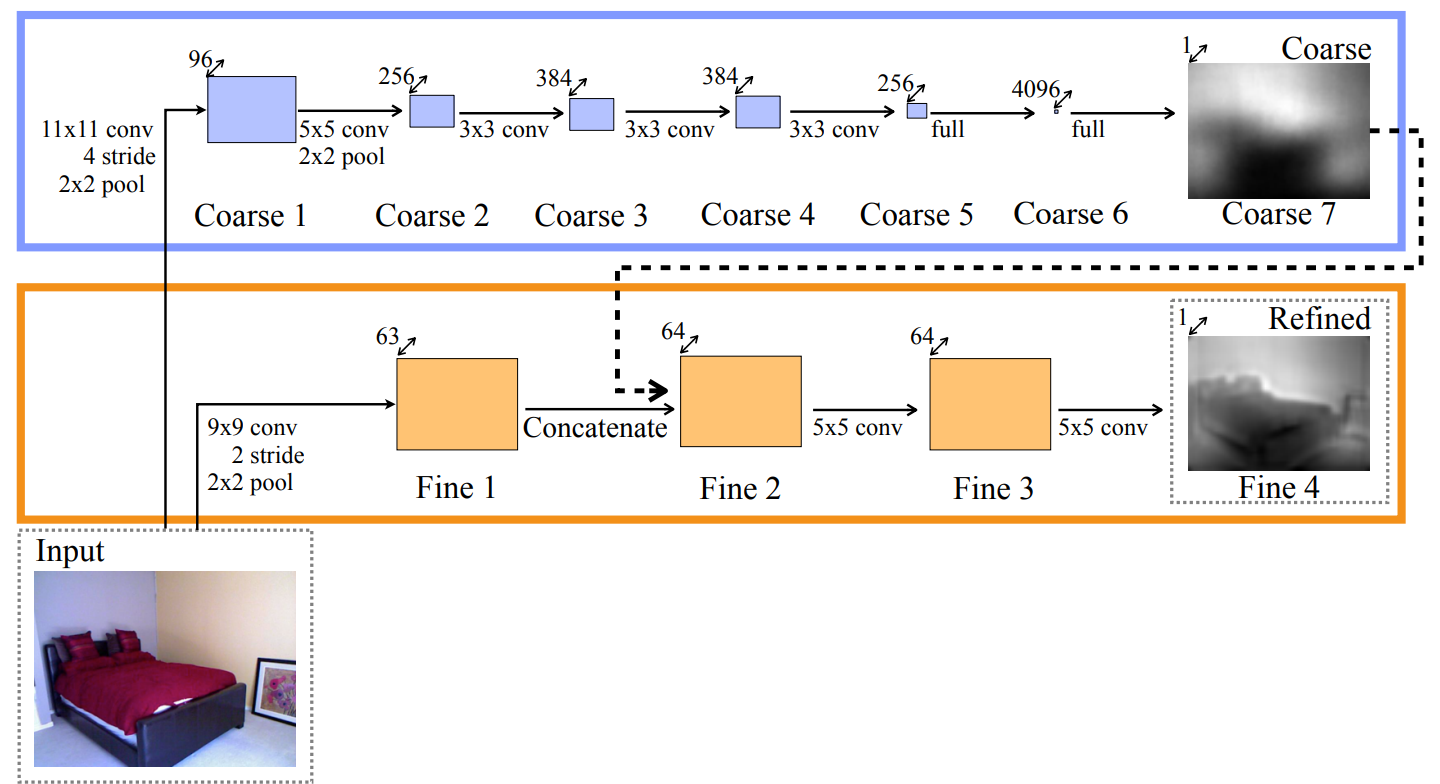
\includegraphics[width=1.\textwidth]{figs/Eigen}
\caption{Eigen et al. \cite{Eigen} two-stage architecture. \label{fig:Eigen}}
\end{figure}

% comments
The networks predict in the \textit{log-scale}, i.e. if $I$ is an input RGB image and $\mathbf{Z}$ is its depth estimate, it can be written:
\begin{equation}
	\begin{split}
	\text{log} \, \mathbf{Z}_{coarse} & = \mathcal{S}_{1}(I) \\
	\text{log} \, \mathbf{Z} & = \mathcal{S}_{2}(I, \, \text{log} \, \mathbf{Z}_{coarse})
	\end{split}
\end{equation}

% loss
Their network is trained using a scale-invariant loss function:
\[
	\delta(i, j) = \text{log} \, \mathbf{Z}^{*} (i, j) - \text{log} \, \mathbf{Z} (i, j)
\]\[
	\mathcal{L}_{scale-invariant} =
	\mathop{\text{mean}}_{(i, j) \in \mathbf{Z}^{*}} \left( \delta(i, j) \right)^{2} \quad +\quad
	\lambda \left( \mathop{\text{mean}}_{(i, j) \in \mathbf{Z}^{*}} \delta(i, j) \right) ^{2}
\]
$\lambda$ is a hyper-parameter that regulates the "scale invariace" of the loss: $\lambda$ set to $0$ reduces $\mathcal{L}_{scale-invariant}$ to a pixel-wise $l^{2}$ loss, $\lambda$ set to $1$ results in the Scale-Invariant Error exactly (introduced in "Metrics" section).
Eigen et al. opt for $\lambda = 0.5$, finding it a good compromise.
Their idea is that if a simple $l^{2}$ loss is used, then the networks probably regress to the mean depth which they proved it accounts for a large error portion.
Conversely, if a pure scale-invariant loss is used, the networks don't learn the metric structure of the scenes.

% architecture 2
\begin{figure}
\centering
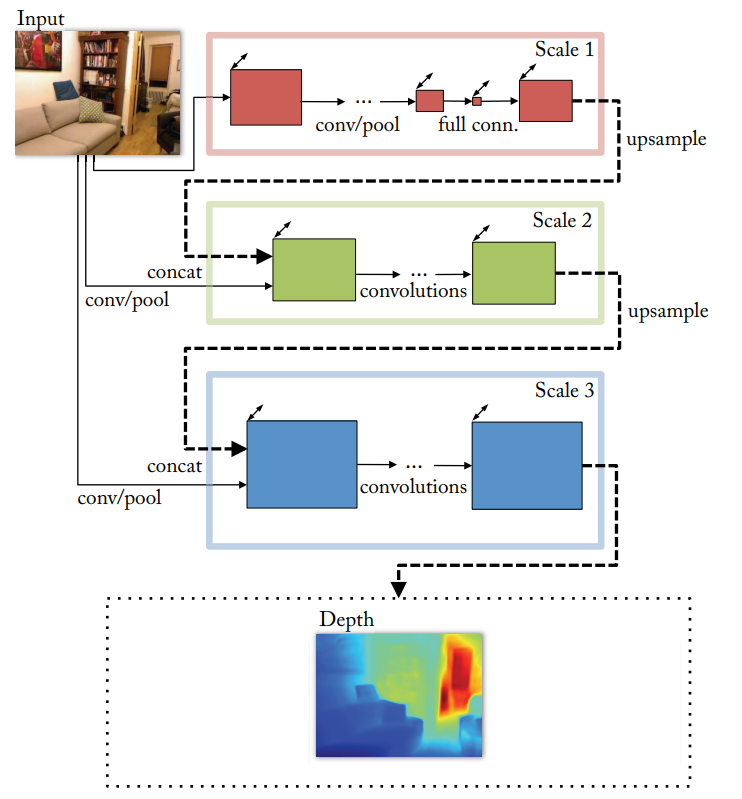
\includegraphics[scale=0.6]{figs/Eigen2}
\caption{Eigen et al. \cite{Eigen2} improved architecture, a third scale network has been added.}
\label{fig:Eigen2}
\end{figure}

% comments
Eigen et al. \cite{Eigen2} improve their previous work \cite{Eigen} by adding a third network $\mathcal{S}_{3}$ ("Scale 3" in \ref{fig:Eigen2}) working on a third finer scale and by substituting the $\mathcal{S}_{1}$ backbone with the larger VGG \cite{VGG}.
The new method has still two stages: the first composed of $\mathcal{S}_{1}$ and $\mathcal{S}_{2}$ and the second is just $\mathcal{S}_{3}$:
\[
	\text{log} \, \mathbf{Z}_{coarse} = \mathcal{S}_{2}(I, \, \mathcal{S}_{1}(I))
\]\[
	\text{log} \, \mathbf{Z} = \mathcal{S}_{3}(I, \, \text{log} \, \mathbf{Z}_{coarse})
\]

% regularization
They train their architecture using the same Scale-Invariant loss, but a regularization term is added:
\begin{equation}
\begin{split}
	\mathcal{L}_{reg} & = \mathop{\text{mean}}_{(i, j) \in \mathbf{Z}^{*}}
		\big\|
			\nabla \delta(i, j)
		\big\|_{2}^{2} \\
	& = \mathop{\text{mean}}_{(i, j) \in \mathbf{Z}^{*}}
		\big\|
			\nabla \text{log} \, \mathbf{Z}^{*} (i, j) - \nabla \text{log} \, \mathbf{Z} (i, j)
		\big\|_{2}^{2}
\end{split}
\end{equation}
This term encourages the predicted depth map to have a local structure similar to the ground-truth one by forcing predicted and ground-truth gradients to be similar (in an $l^{2}$ sense).

%%%%%%%%%%%%%%%%%%%%%%%%%%%%%%%%%%%%%%%%%
%                 LAINA
%%%%%%%%%%%%%%%%%%%%%%%%%%%%%%%%%%%%%%%%%
\subsection{Laina et al.}
Laina et al. \cite{Laina} use a fully convolutional neural network (FCNN) for regressing metric depth maps.
Their architecture is an encoder-decoder based on ResNet \cite{ResNet} and four up-sampling blocks (see figure \ref{fig:Laina}) are introduced and tested for the decoding part.
A great improvement over the work of Eigen et al. is that using an FCNN drastically reduces the number of parameters of the network, making it feasible to increase the output resolution and to work in real-time.
One difference is that Laina et al. network regresses the depth map in linear-scale and not log-scale as Eigen et al. did.

% architecture
\begin{figure}
\centering
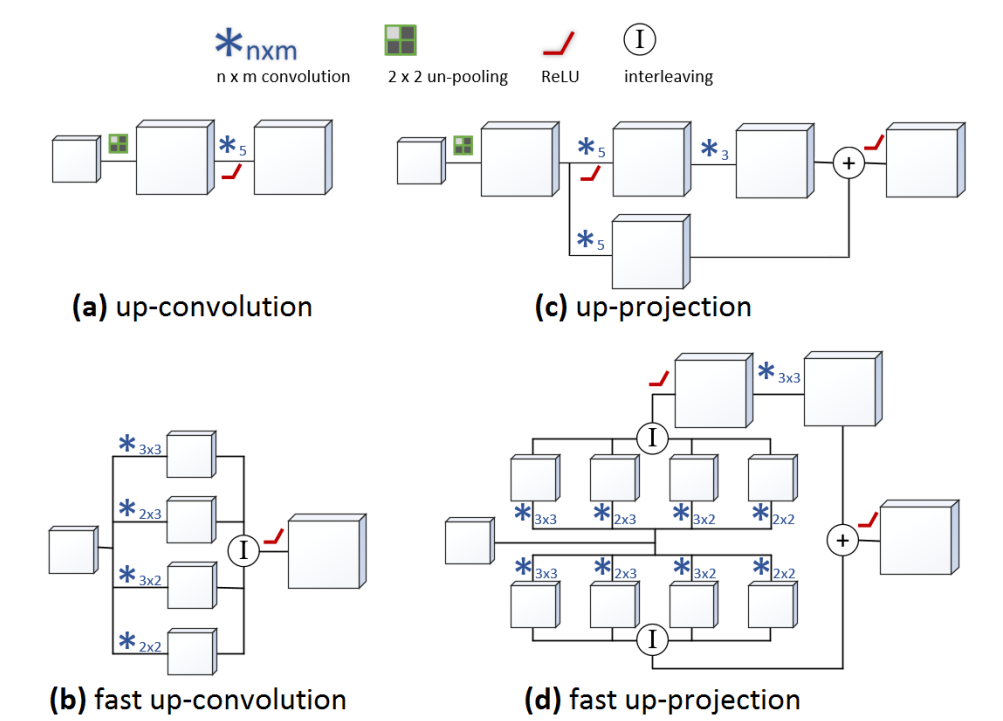
\includegraphics[scale=0.4]{figs/Laina}
\caption{Laina et al. \cite{Laina} up-sampling blocks inspired by ResNet blocks. To be read from left to right. They stack "Fast up-projection" blocks in their decoder. \label{fig:Laina}}
\end{figure}

% loss
For training their network they use the reverse Huber loss (berHu):
\begin{equation}
	\mathcal{B}(x) = 
	\begin{cases}
		|x| & \text{if } |x| \leq c \\
		\frac{x^{2} + c^{2}}{2c} & \text{if } |x| > c
	\end{cases}
\end{equation}
\[
	\mathcal{L}_{berHu} = \mathop{\text{mean}}_{(i, j) \in \mathbf{Z}^{*}} \mathcal{B}(\mathbf{Z}(i, j) - \mathbf{Z}^{*}(i, j))
\]
$\mathcal{B}$ is formulated in such a way that it is continuous and differentiable.
It behaves like an $l^{1}$ loss function in $[-c, c]$ and like an $l^{2}$ loss function outside that interval.
Laina et al. define $c$ batch-wise so that it is 20\% of the maximal per-batch error:
\[
	c = \frac{1}{5} \mathop{\text{max}}_{
		\substack{
			(\mathbf{Z}, \mathbf{Z}^{*}) \in \text{batch} \\
			(i, j) \in \mathbf{Z}^{*}
		}
	} \big| \mathbf{Z}(i, j) - \mathbf{Z}^{*}(i, j) \big|
\]
This is just an empirical heuristic they tuned, other choices for $c$ are also possible.
The authors motivate this loss function by noticing that depth values follow a heavy-tailed distribution (e.g. a log-normal distribution) and berHu loss is thus better suited considering that they work in linear-scale.
This could also explain \cite{Laina} why working in the log-scale was beneficial for Eigen et al., since the logarithm of a log-normal random variable follows a normal distribution which is in general well-behaved.

%%%%%%%%%%%%%%%%%%%%%%%%%%%%%%%%%%%%%%%%%
%                 DIW
%%%%%%%%%%%%%%%%%%%%%%%%%%%%%%%%%%%%%%%%%
\subsection{DIW}
Chen et al. \cite{DIW} tackle \textit{relative} depth estimation in the wild.
They both propose a method for training a model to learn relative depth and introduce a new dataset "Depth in the Wild" (\texttt{DIW}) which is discussed in the "Datasets" section.
The former is here treated.

First they consider an encoder-decoder architecture with long range skip connections as shown in figure \ref{fig:DIW_architecture}.
They take it from other authors and modify it using Inception blocks \cite{Inception}.

% architecture
\begin{figure}
\centering
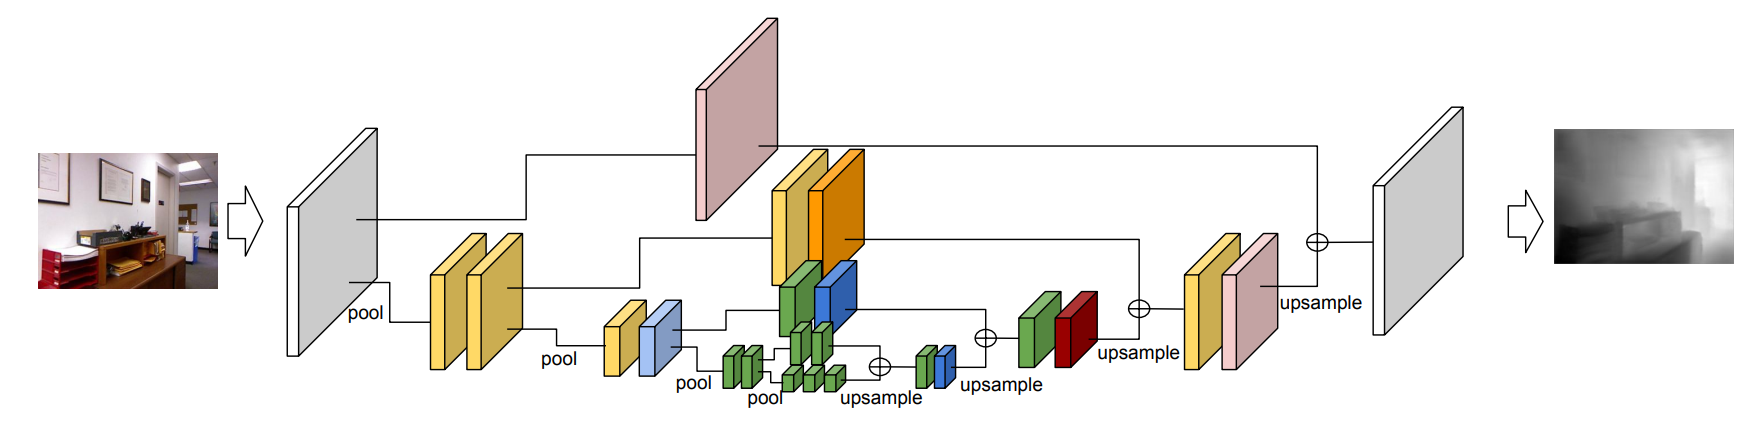
\includegraphics[scale=0.4]{figs/DIW_architecture}
\caption{Chen et al. \cite{DIW} architecture. \label{fig:DIW_architecture}}
\end{figure}

% comments
As they point out, their training method is not architecture-dependent and therefore other choices can be made.
The important thing is that their network outputs a depth map $\mathbf{Z}$ of its input image, this depth map is to be rather interpreted as \textit{relative}, meaning that it can be \textit{only} used for comparing depths between pairs of pixels.
For instance if $\mathbf{p_{1}}$ and $(k,l)$ are two pixels, $\mathbf{Z}(i, j) > \mathbf{Z}(k,l)$ implies that $\mathbf{Z}^{*}(i, j) > \mathbf{Z}^{*}(k,l)$.
Formally a relative depth map equals its metric depth map up to a pixel-wise monotonic transformation\footnote{For this reason, relative depth maps are not expressed in a specified scale, unlike metric depth map which can be expressed in linear-scale, log-scale, ...}.

% loss
For training such a network they employ a \textit{ranking loss} which encourages pairs of pixels to be ordered in a certain way.
Hence, they sample $K$ pairs of pixels from the ground-truth metric depth map and based on their relative depth adjust the predicted relative depth map in those locations:
\[
	\mathcal{L}_{ranking} = \mathop{\text{mean}}_{
		\substack{
			\text{sample } K \text{ pairs}\\
			 \mathbf{p}^{*}_{1} \neq \mathbf{p}^{*}_{2} \in \mathbf{Z}^{*}}
		}
	\begin{cases}
		\text{log} \, ( 1 + \text{exp} \, ( \mathbf{Z}(\mathbf{p}^{*}_{1}) - \mathbf{Z}(\mathbf{p}^{*}_{2}) )) &
			\text{if } \mathbf{Z}^{*}(\mathbf{p}^{*}_{1}) \ll \mathbf{Z}^{*}(\mathbf{p}^{*}_{2}) \\
		\text{log} \, ( 1 + \text{exp} \, ( \mathbf{Z}(\mathbf{p}^{*}_{2}) - \mathbf{Z}(\mathbf{p}^{*}_{1}) )) &
			\text{if } \mathbf{Z}^{*}(\mathbf{p}^{*}_{2}) \ll \mathbf{Z}^{*}(\mathbf{p}^{*}_{1}) \\
		(\mathbf{Z}(\mathbf{p}^{*}_{1}) - \mathbf{Z}(\mathbf{p}^{*}_{2}) )^{2} &
			\text{if } \mathbf{Z}^{*}(\mathbf{p}^{*}_{1}) \approx \mathbf{Z}^{*}(\mathbf{p}^{*}_{2})
	\end{cases}
\]
For deciding whether $\mathbf{Z}^{*}(\mathbf{p}^{*}_{1})$ and  $\mathbf{Z}^{*}(\mathbf{p}^{*}_{2})$ are $\ll$, $\gg$ or $\approx$ they use a dataset-dependent threshold $\tau$:

\begin{align*}
	\mathbf{Z}^{*}(\mathbf{p}^{*}_{1}) & \ll \mathbf{Z}^{*}(\mathbf{p}^{*}_{2}) \quad
		\text{if } \mathbf{Z}^{*}(\mathbf{p}^{*}_{1}) < \mathbf{Z}^{*}(\mathbf{p}^{*}_{2}) - \tau\\
	\mathbf{Z}^{*}(\mathbf{p}^{*}_{1}) & \gg \mathbf{Z}^{*}(\mathbf{p}^{*}_{2}) \quad
		\text{if } \mathbf{Z}^{*}(\mathbf{p}^{*}_{1}) > \mathbf{Z}^{*}(\mathbf{p}^{*}_{2}) + \tau\\
	\mathbf{Z}^{*}(\mathbf{p}^{*}_{1}) & \approx \mathbf{Z}^{*}(\mathbf{p}^{*}_{2}) \quad
		\text{if } |\mathbf{Z}^{*}(\mathbf{p}^{*}_{1}) - \mathbf{Z}^{*}(\mathbf{p}^{*}_{2})| \leq \tau
\end{align*}

It's very unlikely that two distinct pixels share the same identical depth value, thus the equality definition must be relaxed.

%%%%%%%%%%%%%%%%%%%%%%%%%%%%%%%%%%%%%%%%%
%                 ReDWeb
%%%%%%%%%%%%%%%%%%%%%%%%%%%%%%%%%%%%%%%%%
\subsection{ReDWeb}
Xian et al. \cite{ReDWeb} continue to study the problem of monocular relative depth estimation in the wild in the same way as Chen et al. \cite{DIW} did: they introduce a new dataset "Relative Depth from Web" (\texttt{ReDWeb}) and propose a training methodology.
The focus of this discussion is on the latter.
Contrary to \cite{DIW}, here the authors put more emphasis on the design of the architecture they use which is shown in figure \ref{fig:ReDWeb_architecture} below.

% architecture
\begin{figure}
\centering
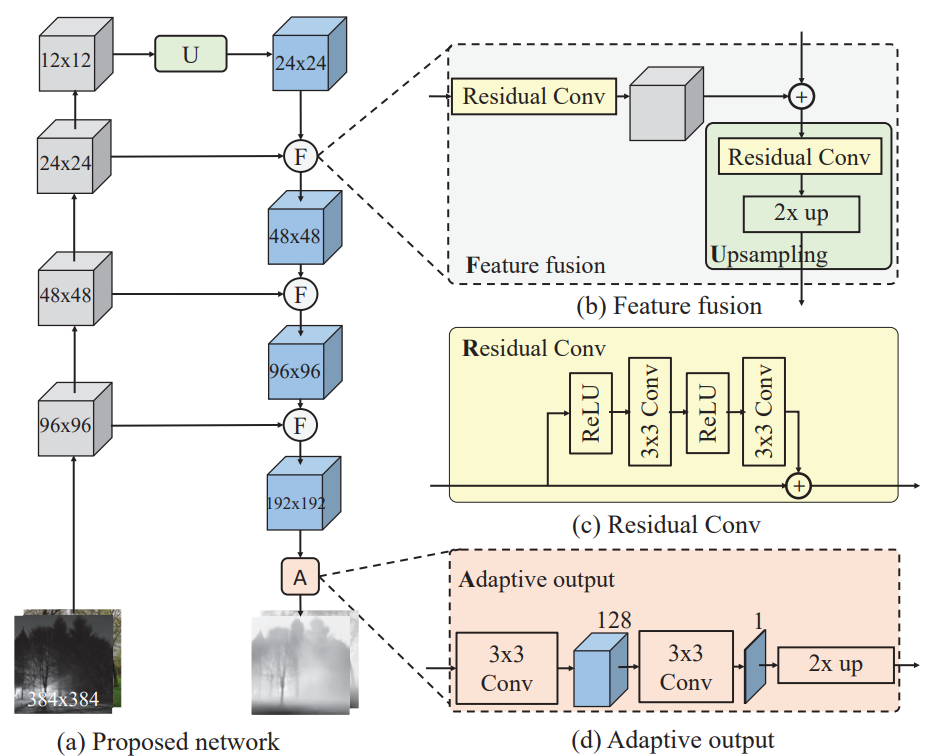
\includegraphics[scale=0.4]{figs/ReDWeb_architecture}
\caption{Xian et al. \cite{ReDWeb} architecture, the encoder backbone is based on ResNet \cite{ResNet} adding a multi-scale fusion module (b) connecting encoded feature maps with decoded ones. \label{fig:ReDWeb_architecture}}
\end{figure}

The idea of their training method is the same of Chen et al., the difference is in the choice of pixel pairs to analyze per image: in \cite{DIW} they were fixed per image, here instead are online sampled.
The sampling procedure produces imbalanced ordinal relations where the number of equal relation is far less than the other two relations.
The solution proposed by Xian et al. is to ignore the pixel pairs that result in the smallest loss and trim the 25\% of sampled pairs that less contribute to the loss function.
In this way two things are achieved: the ratio of the equal relation in the sampling increases and the network is enforced to focus on \textit{hard} pairs during training.

%%%%%%%%%%%%%%%%%%%%%%%%%%%%%%%%%%%%%%%%%
%               denseViT
%%%%%%%%%%%%%%%%%%%%%%%%%%%%%%%%%%%%%%%%%
\subsection{denseViT}
In \cite{denseViT} Ranftl et al. use the ViT \cite{ViT} architecture for monocular affine depth estimation following the MiDas training procedure \cite{MiDas}, their architecture is called Dense Prediction Transformer (DPT).
They substitute the usual fully convolutional encoder with ViT blocks, see figure \ref{fig:denseViT_architecture}.
The main idea is to process image patches using ViT modules and to re-assemble the obtained tokens as their respective patches creating a feature map.
In this way ViT blocks can be combined with usual techniques as convolutions and transposed convolutions for the decoding phase.
Ranftl et al. follow the usual U-Net \cite{UNet} scheme building an encoder-decoder architecture with information flowing from shallow layers of the encoder to deeper layers of the decoder.
The general architecture is represented in \ref{fig:denseViT_architecture}.
Thanks to the MiDas \cite{MiDas} training scheme and the very large meta-dataset (1.4 M images) \texttt{MIX 6} they introduced, DPT reaches and surpasses "state of the art" methods of the time.
Transformers have been known to better scale with dataset size than CNN based architectures do and Ranftl et al. work leverages on this fact \cite{ViT}.

% architecture
\begin{figure}
\centering
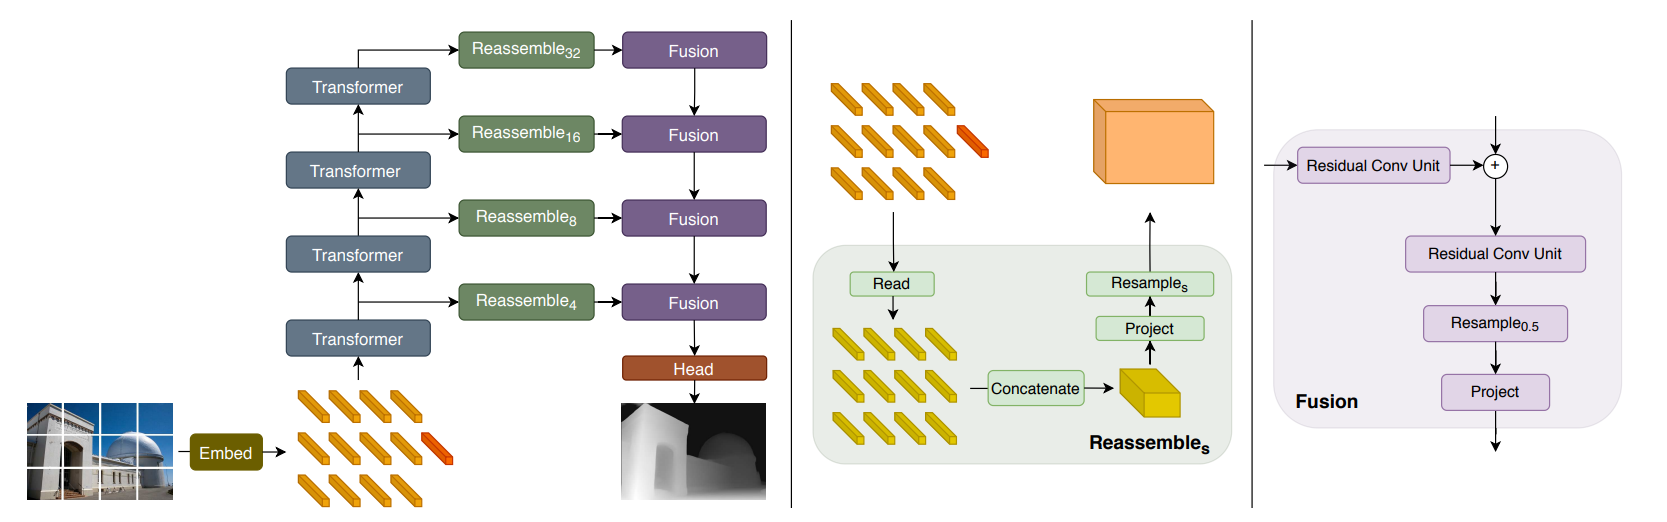
\includegraphics[scale=0.3]{figs/denseViT_architecture}
\caption{Ranftl et al. architecture \cite{denseViT}. \textit{Left}: the general architecture; \textit{Center}: how encoded tokens are processed to get a feature map; \textit{Right}: how multi-scale feature maps are fused during the decoding phase. \label{fig:denseViT_architecture}}
\end{figure}

%%%%%%%%%%%%%%%%%%%%%%%%%%%%%%%%%%%%%%%%%%%%%%%%%%%%%%%%%%%%%%%%%%%%%%%%
\section{Bin Methods}
\label{s:bin_methods}
Instead of regressing continuous depth values, these methods discretize the depth range and work with bins.
The discretization of depth range can be global and fixed \cite{depth_as_classification, ordinal_regression}, global but dependent on the image \cite{AdaBins}, local and dependent on the single pixel \cite{ZoeDepth}.
When probabilities (or scores, depending on the interpretation) are assigned to each bin, a depth value is actually computed which can eventually space in the whole range considered.
Find a summary in \ref{table:2}.

% summary table
\begin{center}
	\begin{table}
		\begin{tabular}{| c | c | c | c | c |}
		\hline
		\textbf{Year} & \textbf{Authors} & \textbf{Task} & \textbf{Formulation} & \textbf{Technique} \\
		\hline
		2018 &  Cao et al. \cite{depth_as_classification} & Metric DE & classification & CNN + CRF \\
		2018 & Fu et al. \cite{ordinal_regression} & Metric DE & ordinal regression & CNN \\
		2021 & Bhat et al. \cite{AdaBins} & Metric DE & hybrid regression & CNN + ViT\\
		2023 & Bhat et al. \cite{ZoeDepth} & Relative + Metric DE & hybrid regression & CNN + ViT\\
		\hline
		\end{tabular}
	\caption{Summary of treated bin methods for depth estimation. \label{table:2}}
	\end{table}
\end{center}

%%%%%%%%%%%%%%%%%%%%%%%%%%%%%%%%%%%%%%%%%
%        Depth as Classification
%%%%%%%%%%%%%%%%%%%%%%%%%%%%%%%%%%%%%%%%%
\subsection{Cao et al.}
Cao et al. \cite{depth_as_classification} formulate depth estimation as a pixel-wise classification task proposing a two-stage method.
Their idea is to discretize depth dividing its range into uniform bins.
The overall pipeline is illustrated in figure \ref{fig:depth_as_classification}

% architecture
\begin{figure}
	\centering
	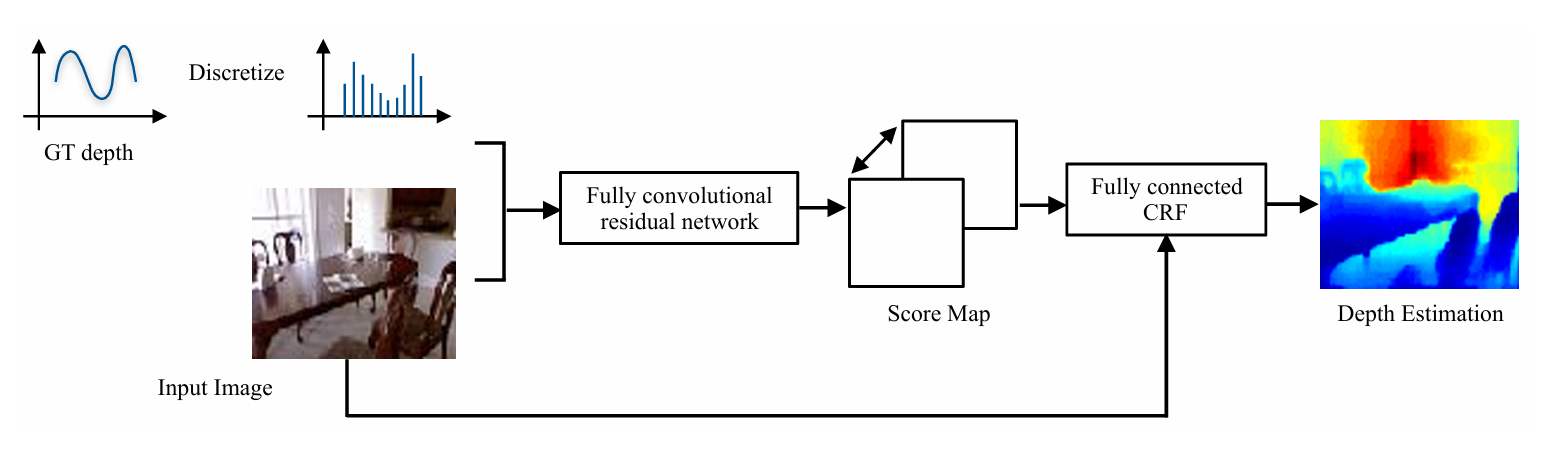
\includegraphics[scale=0.35]{figs/depth_classification}
	\caption{Cao et al. architecture \cite{depth_as_classification}. \label{fig:depth_as_classification}}
\end{figure}

% depth discretization
After an empirical investigation they decide to equally discretize the ground-truth \textit{log} depth range into $B$ bins.
Hence, assuming depth values range between $Z_{\text{min}}$ and $Z_{\text{max}}$, they consider $B+1$ points:
\[
	Z_{\text{min}}=Z_{0} < Z_{1} < Z_{2} < \dotsc < Z_{B} = Z_{\text{max}}
\]\[
	\text{such that} \quad \text{log} \, Z_{b+1} - \text{log} \, Z_{b} =
	\frac{\text{log} \, Z_{\text{max}} - \text{log} \, Z_{\text{min}}}{B}
	\quad b = 0, 1, \dotsc, B-1
\]

% prediction pipeline
The first stage of their method computes for each pixel the probability that its depth falls within a certain bin: if $\mathbf{Z}^{*}$ is the ground-truth depth map, for each pixel $(i, j) \in \mathbf{Z}^{*}$ they give an estimate of:
\[
	\mathbf{P}^{*}_{b}(i, j) = \mathbb{P} \, \{\mathbf{Z}^{*}(i, j) \text{ is between } Z_{b} \text{ and } Z_{b+1}\} \quad b = 0, 1, \dotsc, B-1
\]
This is achieved by a ResNet \cite{ResNet} backbone trained to output a probability map $\mathbf{P}$ of size $W \times H \times B$ with as many channels as bins and a resolution reduced by a factor of 8 w.r.t. the initial image $\mathbf{I}$ of size $W \times H \times 3$ taken as input.
This is then up-sampled by means of bilinear interpolation to the image size.
To obtain probability distributions, a softmax function is applied pixel-wise across prediction channels.

This estimated probability distribution map is converted into a label map:
\[
	\mathbf{L}(i, j) = \mathop{\text{arg max}}_{b \in \{ 0, \dotsc, B-1\}} \mathbf{P}_{b}(i, j)
\]

% loss
The loss employed is a variant of the multinomial logistic loss.
Assume ground-truth depth map $\mathbf{Z}^{*}$ is discretized to its label map $\mathbf{L}^{*}$:
\[
	\mathbf{L}^{*}(i, j) = b \text{ such that } \mathbf{Z}^{*}(i, j) \text{ is in the } b\text{-th bin}
\]
The loss can be expressed as:
\[
	\mathcal{L} =
		- \mathop{\text{mean}}_{(i, j) \in \mathbf{L}^{*}}
		\sum_{b = 0}^{B-1}
		e^{-(b - \mathbf{L}^{*}(i, j))^{2}}
		\text{log} \, \mathbf{P}_{b}(i, j)
\]
The factor $e^{-(b - \mathbf{L}^{*}(i, j))^{2}}$ makes the contribution of a predicted label proportional to its closeness to the ground truth label.
This is meaningful because labels are interpreted as discrete depth values.

% comments on post-processing
Cao et al. use a fully-connected Conditional Random Field (CRF) to post-process the predicted depth label map in the second stage.
Simply put, a CRF is a \textit{global} optimization procedure that adjusts discrete variables to minimize a certain quantity which encodes desired properties.
A fully-connected CRF is a special kind of CRF.
Not going into details, check \cite{computer_vision} for more.

The optimized label map $\mathbf{L}$ must be converted back to a depth map $\mathbf{Z}$.
The authors map labels to their respective bin centers by means of the following formulas:
\[
	\quad c_{b} = \frac{Z_{b} + Z_{b+1}}{2} \quad b = 0, 1, \dotsc, B-1
\]\[
	\mathbf{Z}(i, j) = c_{\mathbf{L}(i, j)}
\]
This sums up \cite{depth_as_classification}.

%%%%%%%%%%%%%%%%%%%%%%%%%%%%%%%%%%%%%%%%%
%        Ordinal Regression
%%%%%%%%%%%%%%%%%%%%%%%%%%%%%%%%%%%%%%%%%
\subsection{Fu et al.}
Fu et al. \cite{ordinal_regression} continue this line of research by adopting a slightly different approach which proved more effective.
They formulate depth estimation as an \textit{ordinal regression} problem.
The formal setting is very similar to the one of Cao et al., I will now illustrate the differences.
First, their method is end-to-end as shown in the image \ref{fig:Fu_ordinal}.

% architecture
\begin{figure}
	\centering
	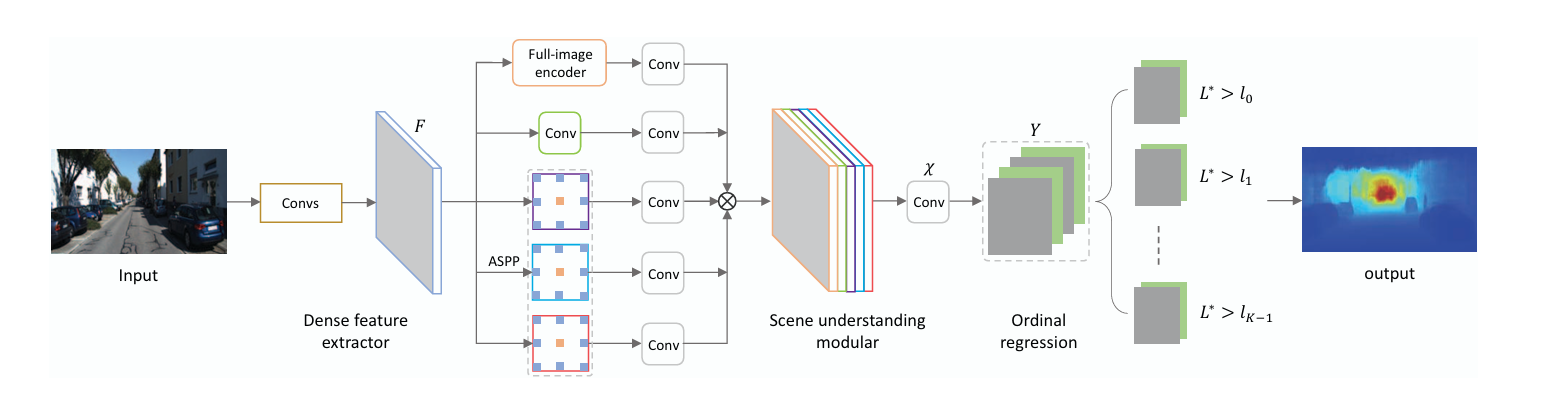
\includegraphics[scale=0.35]{figs/Fu_ordinal}
	\caption{Fu et al. architecture \cite{ordinal_regression}. It employs an "atrous spatial pyramid pooling" module (ASPP) which deals with multiscale details by working with various dilation rates for convolutions. \label{fig:Fu_ordinal}}
\end{figure}

Second, a more sophisticated architecture estimates $\mathbf{P}^{*}$ from $\mathbf{I}$, and it is composed of different modules, some working in parallel and some in serial.
They use dilated convolutions for enlarging the field of view without decreasing spatial resolution or increasing number of parameters \cite{ordinal_regression} and $1 \times 1$ convolutions for cross-channel interactions \cite{ordinal_regression}.
Third, they interpret $\mathbf{P}^{*}_{b}(i, j)$ as $\mathbb{P} \, \{ \mathbf{Z}^{*}(i, j) < Z_{b+1} \}$, namely the probability that the pixel $(i, j)$ corresponds to a point that doesn't fall farther than the $b$-th depth bin.
If a pixel $(i, j)$ corresponds to bin $\mathbf{L}^{*}(i, j)$ then $\mathbf{P}_{b}(i, j)$ must be maximized for $b \leq \mathbf{L}^{*}(i, j)$ and minimized for $b > \mathbf{L}^{*}(i, j)$, hence the following loss function:
\[
	\mathcal{L} = - \mathop{\text{mean}}_{(i, j) \in \mathbf{L}^{*}}
	\left(
		\sum_{b=0}^{\mathbf{L}^{*}(i, j)} \text{log} \,( \mathbf{P}_{b}(i, j)) \quad +
		\sum_{b=\mathbf{L}^{*}(i, j) + 1}^{B-1} \text{log} \, (1 - \mathbf{P}_{b}(i, j))
	\right)
\]
The predicted label map $\mathbf{L}$ is defined as:
\[
	\mathbf{L}(i, j) = | \{b \, \text{ such that } \, \mathbf{P}_{b}(i, j) > 0.5\} |
\]
Ideally $\mathbf{P}_{b}(i, j) > 0.5$ for $b \leq \mathbf{L}^{*}(i, j)$ and $\mathbf{P}_{b}(i, j) \leq 0.5$ for $b > \mathbf{L}^{*}(i, j)$, so that $\mathbf{L}(i, j) = \mathbf{L}^{*}(i, j)$.
In case $\mathbf{P}_{b}(i, j)$ is above $0.5$ for every $b$, $(i, j)$ can be considered at a depth outside the range $Z_{\text{min}}$, $Z_{\text{max}}$, e.g. it can correspond to a point at $\infty$ depth like the sky.

%%%%%%%%%%%%%%%%%%%%%%%%%%%%%%%%%%%%%%%%%
%               AdaBins
%%%%%%%%%%%%%%%%%%%%%%%%%%%%%%%%%%%%%%%%%
\subsection{AdaBins, LocalBins and ZoeDepth}
Shariq Farooq Bhat and other researchers worked a lot on single image depth estimation using bin-methods and developed three important works: AdaBins \cite{AdaBins}, LocalBins \cite{LocalBins} and ZoeDepth \cite{ZoeDepth}.

\paragraph{AdaBins} In the first work, Bhat et al. \cite{AdaBins} generalize the ideas from Fu et al. \cite{ordinal_regression}.
They observe that depth distribution vary to a large extent between different scenes, therefore depth bins must be adapted per image.
The pipeline is illustrated in figure \ref{fig:adabins}.

% architecture
\begin{figure}
	\centering
	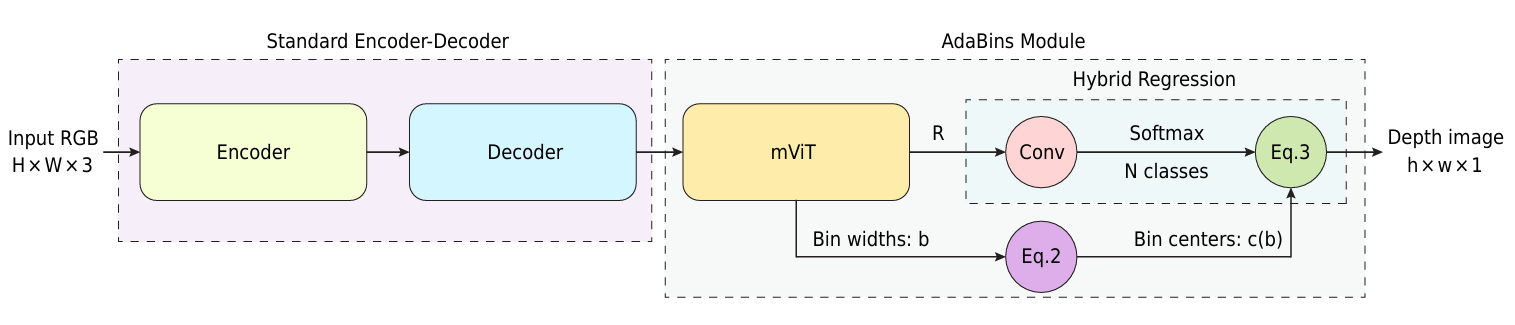
\includegraphics[scale=0.35]{figs/adabins}
	\caption{Bhat et al. architecture \cite{AdaBins}. \label{fig:adabins}}
\end{figure}

The image $\mathbf{I}$ is processed by an encoder $\mathcal{E}$ decoder $\mathcal{D}$ architecture to obtain what the authors call \textit{decoded features}, that is a multichannel feature map $\mathbf{F}$:
\[
	\mathbf{F} = \mathcal{D}(\mathcal{E}(\mathbf{I})) \quad H \times W \times C \text{ feature map}
\]
The rest of the pipeline is the "AdaBins" block, as the authors call it.
The idea of Bhat et al. for estimating the bins adaptively is to extract \textit{global} information and to use that for the purpose.
A Vision Transformer (ViT) \cite{ViT} is used for exploiting global context.
A Vit takes an image as input, divide it into grid patches, process them favouring information exchange and outputs a vector for each of them. Calling the Vit $\mathcal{T}$, the image is divided into $S$ patches:
\[
	\mathcal{T}: \mathbb{R}^{H \times W \times C} \rightarrow \mathbb{R}^{S \times C}
\]
Hence $\mathcal{T}(\mathbf{F}) = (\mathcal{T}(\mathbf{F})_{1}, \dotsc, \mathcal{T}(\mathbf{F})_{S})$ are $S$ vectors of $\mathbb{R}^{C}$.
Each of these vectors encodes global information, any one of them can be used to get the bins, e.g. the first one $\mathcal{T}(\mathbf{F})_{1}$.
The authors construct the discretization of the depth range by computing relative bin-widths from global information:
\[
	(w_{0}, \dotsc, w_{B-1}) = \text{learnable mapping }(\mathcal{T}(\mathbf{F})_{1})
\]\[
	\text{such that } \forall b \,\, w_{b} > 0 \, \text{ and } \, \sum_{b=0}^{B-1} w_{b} = 1
\]
Bins extrema $Z_{b}$ and bin centers $c_{b}$ can be calculated knowing the depth range $Z_{\text{max}}$, $Z_{\text{min}}$ (dataset dependent) and by using the following formula:
\[
	w_{b} = \frac{Z_{b+1} - Z_{b}}{Z_{\text{max}} - Z_{\text{min}}} \quad b=0, 1, \dotsc, B-1
\]
Now that the depth range has been discretized, labels probabilities need to be computed.
For this final step global information is exploited again: $\mathbf{F}$ (which has $C$ channels) is convolved with each $\mathcal{T}(\mathbf{F})_{s}$ $s=1,\dotsc,S$, which are thought as $C \times 1 \times 1$ kernels and an $H \times W \times S$ map is returned which is in turn pixel-wise processed to obtain a probability map $\mathbf{P}$ of size $H \times W \times B$.

Finally, depth can be estimated.
To avoid discretization artifacts they compute the depth as the following linear combination:
\[
	\mathbf{Z}(i, j) = \sum_{b=0}^{B-1} c_{b} \, \mathbf{P}_{b}(i, j)
\]
Therefore, in this work, $\mathbf{P}_{b}(i, j)$ can be interpreted as an approximation to the p.d.f. of the pixel-wise depth distribution.

While for optimizing the depth map obtained Bhat et al. use a Scale-Invariant loss \cite{Eigen}, for optimizing the bin centers $c_{b}$ they adopt the following:
\[
	\mathcal{L}_{\text{bins}} =
	\sum_{(i, j) \in \mathbf{Z}^{*}} \mathop{\text{min}}_{b \in \{0, \dotsc, B-1\}} \, (\mathbf{Z}^{*}(i, j) - c_{b})^{2} \quad+
	\sum_{b \in \{0, \dotsc, B-1\}} \mathop{\text{min}}_{(i, j) \in \mathbf{Z}^{*}} \, (\mathbf{Z}^{*}(i, j) - c_{b})^{2}
\]
This loss, called "bidirectional Chamfer Loss" \cite{AdaBins}, encourages the bin center distribution to match the ground-truth depth distribution.

%%%%%%%%%%%%%%%%%%%%%%%%%%%%%%%%%%%%%%%%%
%              LocalBins
%%%%%%%%%%%%%%%%%%%%%%%%%%%%%%%%%%%%%%%%%

\paragraph{LocalBins} In \cite{LocalBins} Bhat et al. notice that depth discretization must be performed locally, pixel-wise, rather than globally.
In fact, depth values distributions can widely vary across a single image.
The overall procedure is shown in figure \ref{fig:localbins}.

% architecture
\begin{figure}
	\centering
	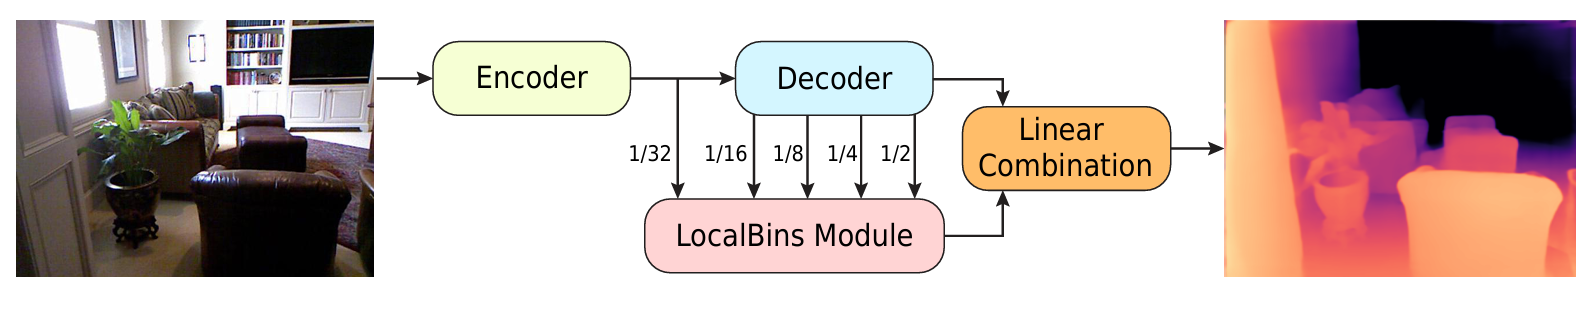
\includegraphics[scale=0.3]{figs/localbins}
	\caption{Bhat et al. architecture \cite{LocalBins}. LocalBins module contains pixel-wise operations and estimate local neighborhood bin density for each pixel location. \label{fig:localbins}}
\end{figure}

Instead of directly predicting the whole depth range discretization, Bhat et al. employ a coarse-to-fine binning strategy.
They start from $B_{\text{seed}}$ bins and during the decoding phase, exploiting multi-scale processing, they apply a bin-splitter module that doubles the number of bins.
Bins are specified through their widths, like in AdaBins, but pixel-wise, so a map $\mathbf{W} \in \mathbb{R}^{H \times W \times B}$ is computed at each step of the decoding phase with $B$ doubling each time.
To "split the bins" the idea is to divide each bin-width into two more by means of a convex combination.
Basically a map $\mathbf{A}$ of same shape as $\mathbf{W}$ is computed but with values in $(0, 1)$ and the new bin-widths are obtained by concatenating the two following tensors:
\[
	\mathbf{B}_{0} = \mathbf{A} \odot \mathbf{W}
\]\[
	\mathbf{B}_{1} = (1 - \mathbf{A}) \odot \mathbf{W}
\]\[
	\mathbf{B}_{\text{new}} = \text{concat} (\mathbf{B}_{0}, \mathbf{B}_{1})
\]
The training loss is similar to the Chamfer loss introduced above, but adapted to the multi-scale setting.
For further details see \cite{LocalBins}.

%%%%%%%%%%%%%%%%%%%%%%%%%%%%%%%%%%%%%%%%%
%              ZoeDepth
%%%%%%%%%%%%%%%%%%%%%%%%%%%%%%%%%%%%%%%%%
\paragraph{ZoeDepth} Eventually, Bhat et al. \cite{ZoeDepth} refine their ideas for computing depth bins pixel-wise in their work called "ZoeDepth".
The result is a two-stage method for estimating both relative and metric depth, the overall architecture is shown in figure \ref{fig:zoe_depth}.

% architecture
\begin{figure}
	\centering
	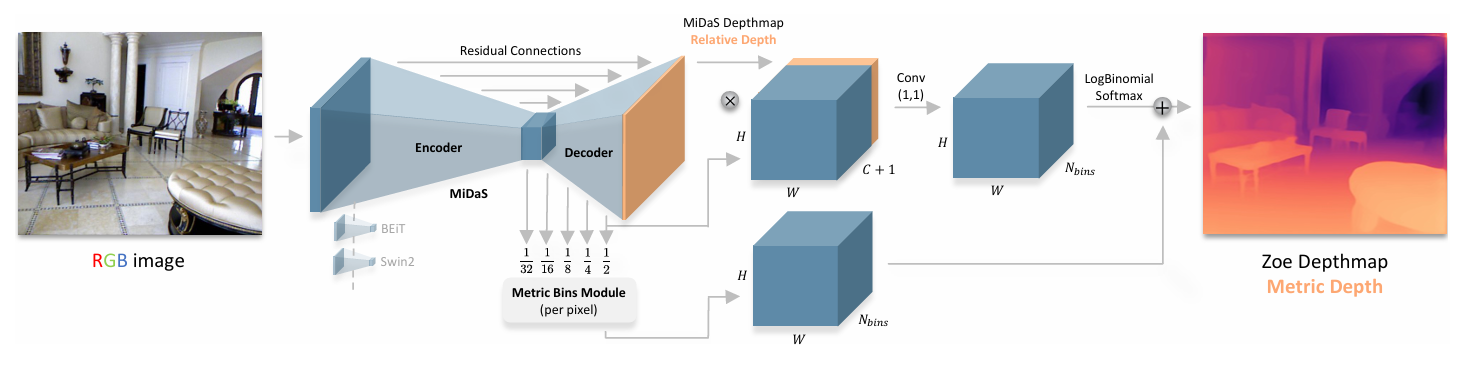
\includegraphics[scale=0.3]{figs/zoe_depth}
	\caption{Bhat et al. architecture \cite{ZoeDepth}. \label{fig:zoe_depth}}
\end{figure}

They use the multi-dataset training procedure of \cite{MiDas} and the general encoder-decoder architecture for estimating relative depth maps is taken from \cite{denseViT}.
To the decoder they attach a head, which they call "Metric Bins Module", for converting relative depth maps into metric depth maps.
Therefore, when training on relative depth datasets only the decoder output is used, whilst when training on metric depth datasets the output of the head is considered.
The Metric Bins Module works at multiple scales: given the lowest scale relative depth map returned by the decoder, a point-wise convolution estimates $B$ bin centers $\{\mathbf{C}_{0}, \mathbf{C}_{1}, \dotsc, \mathbf{C}_{B-1}\} \subset \mathbb{R}^{H \times W \times B}$ pixel-wise, then at successive finer scales other point-wise convolutions return $K$ "attractors" $\{\mathbf{A}_{1}, \mathbf{A}_{2}, \dotsc, \mathbf{A}_{K}\} \subset \mathbb{R}^{H \times W \times K}$, which serve the purpose to modify the previously computed bin distributions pixel-wise by computing an adjustment $\triangle \mathbf{C}_{b}$ for each bin center:
\[
	\triangle \mathbf{C}_{b} = \sum_{k=1}^{K} \frac{\mathbf{A}_{k} - \mathbf{C}_{b}}{1 + \alpha | \mathbf{A}_{k} - \mathbf{C}_{b} |^{\gamma}}
\]
Like before, they assign to each bin (pixel-wise) a probability $\mathbf{P}_{b}$ so that the predicted depth map is:
\[
	\mathbf{Z} = \sum_{i=0}^{B-1} \mathbf{C}_{b} \, \mathbf{P}_{b}
\]
In this formula bins are ordered since their ordering is not preserved during training depending on how the attractors influence.
To make sure not to obtain a difficult to interpret multi-modal probability distributions, the authors build $\mathbf{P}$ pixel-wise and across the bins-channel using the binomial distribution.
Hence, instead of predicting the actual probability values, binomial distribution parameters are computed.
To make things numerically stable they employ some more trickery I won't report.

\newpage
\section{Self Supervised}
There's a line of research tackling monocular depth estimation from a self-supervised learning approach.
Well studied geometric relations implicitly constrain depth maps of subsequent frames in videos or in stereo pairs making it suitable to define self-supervised losses for training, i.e. not dependent on ground truth depth maps.
The general idea is simple: given a pair of images geometrically related (e.g. subsequent video frames or a stereo pair), predict the disparity map of one of them and use it to reconstruct the other, the quality of the reconstruction is the target of the optimization.

%%%%%%%%%%%%%%%%%%%%%%%%%%%%%%%%%%%%%%%%%
%              Garg
%%%%%%%%%%%%%%%%%%%%%%%%%%%%%%%%%%%%%%%%%
\subsection{Garg et al.}
Garg et al. \cite{Garg} rely on having rectified stereo footage with known baseline and camera parameters.
In figure \ref{fig:garg} the training pipeline is illustrated.

% training pipeline
\begin{figure}
	\centering
	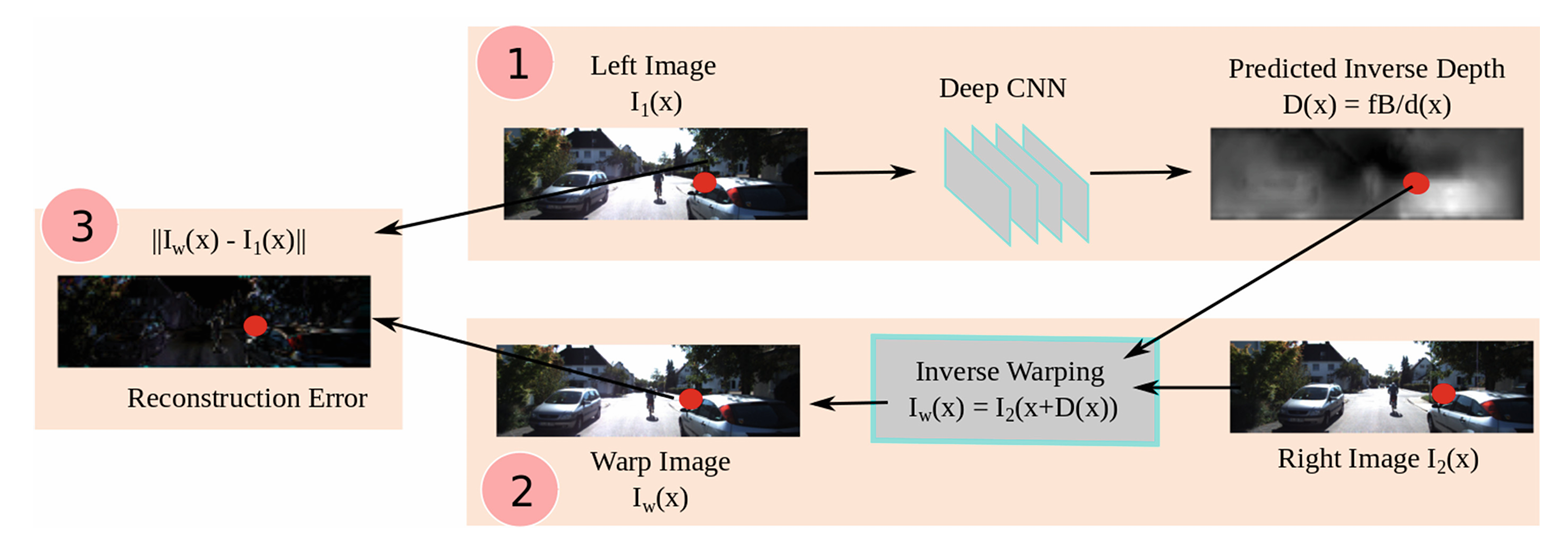
\includegraphics[scale=0.3]{figs/garg}
	\caption{Garg et al. self supervised pipeline \cite{Garg}. \label{fig:garg}}
\end{figure}

Given a stereo pair $\mathbf{I}_{l}, \mathbf{I}_{r}$ they feed $\mathbf{I}_{l}$ to their depth estimation network which returns an estimate of its depth map $\mathbf{Z}_{l}$.
After converting $\mathbf{Z}_{l}$ to a disparity map $\mathbf{D}_{l}$, this can be used to reconstruct the left image using the following formula: $\hat{\mathbf{I}}_{l} (p) = \mathbf{I}_{r} (p + \mathbf{D}_{l}(p))$, for all pixels $p \in \mathbf{D}_{l}$.
A first order approximation of its gradient is provided through an iterative algorithm, this same procedure represents one of the main limitations of this work since it makes the procedure computationally much more expensive.
The loss to be minimized is the reconstruction error between $\hat{\mathbf{I}}_{l}$ and $\mathbf{I}_{l}$, Garg et al. define it as a mean squared error:
\[
	\mathcal{L}_{rec} = \text{mean}_{p \in \hat{\mathbf{I}}_{l}} \big\| \hat{\mathbf{I}}_{l}(p) - \mathbf{I}_{l}(p) \big\|^{2}
\]
The authors also employ a regularization term that smooths the resulting disparity maps:
\[
	\mathcal{L}_{smooth} = \text{mean}_{p \in \hat{\mathbf{I}}_{l}} \big\| \nabla \mathbf{D}_{l} (p) \big\|^{2}
\]

%%%%%%%%%%%%%%%%%%%%%%%%%%%%%%%%%%%%%%%%%
%              MonoDepth
%%%%%%%%%%%%%%%%%%%%%%%%%%%%%%%%%%%%%%%%%
\subsection{MonoDepth}
Godard et al. \cite{MonoDepth} builds upon the work of Garg et al. \cite{Garg}.
Their method is called MonoDepth.

Let's consider the pair of images captured by a stereo cameras $(\mathbf{I}^{l}, \mathbf{I}^{r})$, their disparity maps $(\mathbf{D}^{l}, \mathbf{D}^{r})$?

Consider a pixel $p$ in the left image $\mathbf{I}^{l}$, this corresponds to a position in the scene 3D space.
This same scene is captured from a different view point by the right camera, the result is the right image $\mathbf{I}^{r}$.
There is a pixel of the right image that corresponds to the pixel $p$ of the left image, meaning that they represent the same location in the scene 3D space and their color is identical.
If we overlap $\mathbf{I}^{l}$ and $\mathbf{I}^{r}$ we can see the displacement between the two pixels, which can be represented as a 2D vector and let's call it $\mathbf{D}^{l}(p)$, so we get:
\[
	\mathbf{I}^{l}(p) = \mathbf{I}^{r}(p + \mathbf{D}^{l}(p))
\]

$\mathbf{D}^{l}(p)$ is the offset to apply to $p$ location in the left image in order to obtain its corresponding location in the right image, hence $\mathbf{D}^{l}$ is a 2D vector field of shape $H \times W \times 2$.
This is the left disparity map, symmetrically for the right disparity map it holds:
\[
	\mathbf{I}^{r}(p) = \mathbf{I}^{l}(p + \mathbf{D}^{r}(p))
\]
By means of this very symmetry, one disparity map can be written in terms of the other:
\[
\mathbf{D}^{l}(p) = - \mathbf{D}^{r}(p + d(p)^{l})
\]\[
\mathbf{D}^{r}(p) = - \mathbf{D}^{l}(p + d(p)^{r})
\]

Now, not every 3D scene location can be visible from all view-points since occlusion can happen.
Thus, disparity maps are not defined at every pixel location.
Another assumption that was made during this discussion is that object appearance is view-point independent, this only holds for Lambertian surfaces and if we do not consider atmospheric effects.
This assumption led to corresponding pixels in different images have the same color.
But since it is useful, the Godard et al. keep it.

As stated before, Godard et al. apply their method to \textit{rectified} stereo footage, what is that?
It's just video footage captured by stereo cameras which are aligned in such a way that disparity vectors are always horizontal, hence the 2D disparity vector field reduces to a 1D vector field, i.e. of shape $H \times W$.

Assume now that the right image is unknown, given the right disparity map it can be reconstructed in a \textit{differentiable} manner by following the above formulas.
Similarly, for the left image the procedure is the same given the left disparity map.
The limitation of Garg et al. work is now surpassed by employing a simpler sampling procedure for reconstruction that comes from "Spatial Transformer Network" paper \cite{STN}.
This makes the gradient computation exact and cheaper.

If $\mathbf{I}^{l}$ and $\mathbf{D}^{l}$ are given and \textit{stereo baseline and camera parameters are known}, the depth map of $\mathbf{I}^{l}$ can be computed.
Refer to \cite{multiview} for the general case, but in the rectified case is simple trigonometry.
A network for estimating $\mathbf{D}^{l}$ and $\mathbf{D}^{r}$ from $\mathbf{I}^{l}$ is trained.
The estimation of both disparity maps enforces additional consistency.

The loss function to be minimized per image pair is the following:
\[
	\mathcal{L} = \alpha_{ap}(\mathcal{L}_{ap}^{l} + \mathcal{L}_{ap}^{r}) +
		\alpha_{ds}(\mathcal{L}_{ds}^{l} + \mathcal{L}_{ds}^{r}) +
		\alpha_{lr}(\mathcal{L}_{ds}^{l} + \mathcal{L}_{lr}^{r}) 
\]
Where $\alpha_{ap}$, $\alpha_{ds}$, $\alpha_{lr}$ are positive hyperparameters.
While $\mathcal{L}_{ap}$ is the image reconstruction error, $\mathcal{L}_{ds}$ and $\mathcal{L}_{lr}$ are two regularization terms enforcing more geometric consistency in the predicted disparity maps.

\textbf{Appearance Matching Loss} $\mathcal{L}_{ap} \quad$ This is a photometric image reconstruction loss, meaning that penalizes pairs of images appearing too different locally.
How to measure similarity in appearance?
In \cite{SSIM} Wang et al. developed a differentiable similarity index for comparing the appearance of two image patches called \textsc{SSIM}.
In here Godard et al. couple it with the $L1$ loss to account for appearance discrepancies.
\[
	\mathcal{L}_{ap}^{l} = \textsc{Mean}_{p \in \mathbf{I}^{l}}
		\left(
			0.85 \frac{
				1 - \textsc{SSIM} (\mathbf{I}^{l}(p), \hat{\mathbf{I}}^{l}(p))
			}{2} +
			0.15 \big| \mathbf{I}(p)^{l} - \hat{\mathbf{I}}(p)^{l} \big|
		\right)
\]\[
	\mathcal{L}_{ap}^{r} = \textsc{Mean}_{p \in \mathbf{I}^{r}}
		\left(
			0.85 \frac{
				1 - \textsc{SSIM} (\mathbf{I}^{r}(p), \hat{\mathbf{I}}^{r}(p))
			}{2} +
			0.15 \big| \mathbf{I}(p)^{r} - \hat{\mathbf{I}}(p)^{r} \big|
		\right)
\]

\textbf{Disparity Smoothness Loss} $\mathcal{L}_{ds} \quad$ Except for edges and holes in the disparity map, we expect it to be smooth.
How to mathematically express this?
Smoothness (not in the mathematical sense) means a gradient low in magnitude, so that there are not abrupt changes.
The exception is on the edges, which can be loosely characterized as the points with high magnitude image gradient.
By multiplying $\big| \partial \mathbf{D}(p) \big|$ by $e^{- \big| \partial \mathbf{I}(p) \big| }$smoothness is enforced only on the "interior".
Adapting this idea to the fact that images have 3 channels and the gradient operator has two components, the result is:
\[
	\mathcal{L}_{ds}^{l} = \textsc{Mean}_{p \in \mathbf{I}^{l}}
		\left(
			\big| \partial_{x} \mathbf{D}^{l}(p) \big| e^{-\big\| \partial_{x} \mathbf{I}^{l}(p) \big\| } + 
			\big| \partial_{y} \mathbf{D}^{l}(p) \big| e^{-\big\| \partial_{y} \mathbf{I}^{l}(p) \big\| }
		\right)
\]\[
	\mathcal{L}_{ds}^{r} = \textsc{Mean}_{p \in \mathbf{I}^{r}}
		\left(
			\big| \partial_{x} \mathbf{D}^{r}(p) \big| e^{-\big\| \partial_{x} \mathbf{I}^{r}(p) \big\| } + 
			\big| \partial_{y} \mathbf{D}^{r}(p) \big| e^{-\big\| \partial_{y} \mathbf{I}^{r}(p) \big\| }
		\right)
\]

\textbf{Left-Right Disparity Consistency Loss} $\mathcal{L}_{lr} \quad$ This enforces disparity maps to obey above relations.
Notice that even though the losses in the left and right images are perfectly symmetrical, there are image locations in which only one of them makes sense because the other exceeds image boundaries.
Hence, both of them are needed.
\[
	\mathcal{L}_{lr}^{l} = \textsc{Mean}_{p \in \mathbf{I}^{l}}
		\left(
			\big| \mathbf{D}^{l}(p) + \mathbf{D}^{r}(p + \mathbf{D}^{l}(p)) \big|
		\right)
\]\[
	\mathcal{L}_{lr}^{r} = \textsc{Mean}_{p \in \mathbf{I}^{r}}
		\left(
			\big| \mathbf{D}^{r}(p) + \mathbf{D}^{l}(p + \mathbf{D}^{r}(p)) \big|
		\right)
\]
This ends the treatment of this paper.

%%%%%%%%%%%%%%%%%%%%%%%%%%%%%%%%%%%%%%%%%
%              SfMLearner
%%%%%%%%%%%%%%%%%%%%%%%%%%%%%%%%%%%%%%%%%
\subsection{SfMLearner}
Requiring stereo footage for training is a bit of a request, what if simple monocular video footage could be used?
Zhou et al. solve this problem in \cite{SfMLearner} by only asking camera intrinsics to be known.
Their idea is to extract stereo pairs from a monocular video footage.
In fact, if the scene is static and subsequent frames are taken from different angles then these frames can be thought as a stereo pair.
The next step is to estimate the unknown camera transformation between the two frames.
The figure \ref{fig:sfmlearner} shows the general procedure called SfMLearner (Structure from Motion Learner).

% training pipeline
\begin{figure}
	\centering
	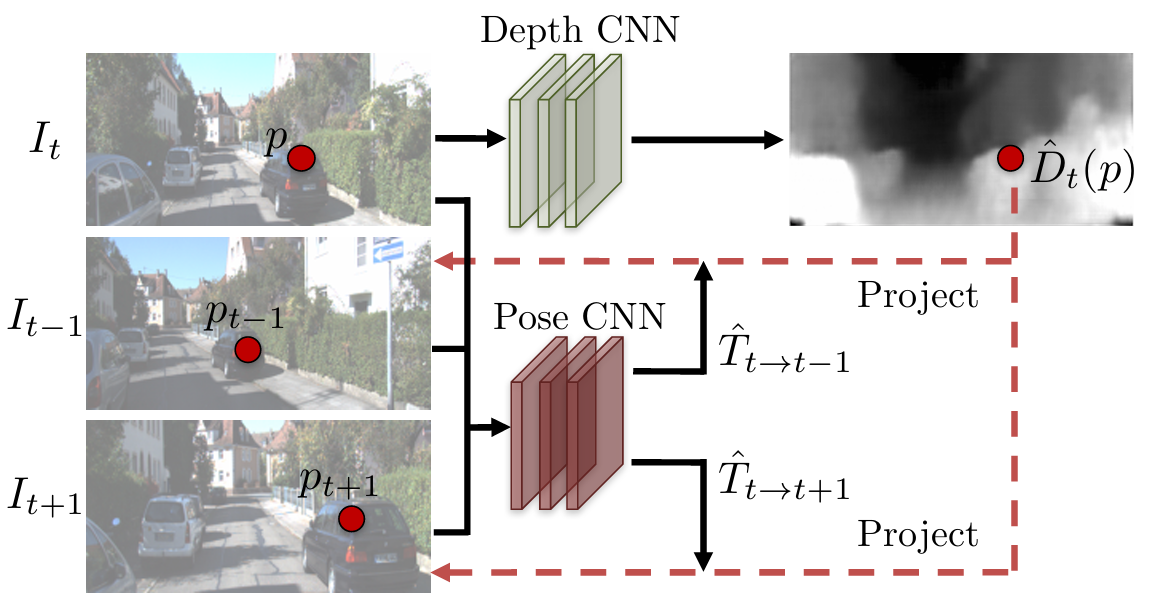
\includegraphics[scale=0.3]{figs/sfmlearner}
	\caption{Zhou et al. self supervised pipeline \cite{SfMLearner} that uses monocular video footage. \label{fig:sfmlearner}}
\end{figure}

Starting simple: if an image $\mathbf{I}$, its depth map $\mathbf{Z}$ and the camera intrinsics matrix $\mathbf{K}$ are given, then each pixel location $p$ can be \textit{differentiably} back-projected to its scene 3D space location $\mathbf{x}$ (refer to \cite{multiview} as usual).
$\mathbf{x}$ is expressed w.r.t. the camera reference frame.
If the camera is moved through a rigid transformation $\mathcal{T}$ (i.e. translation and rotation) then $\mathcal{T}^{-1} (\mathbf{x})$ are the coordinates w.r.t. the new reference frame.
The updated $\mathbf{x}$ can now be projected to the new image plane.
This procedure can be used to reconstruct one image from the other, given the depth map of one of them.
Zhou et al. call "\textit{target} frame" the one to reconstruct and "\textit{source} frame" the one used for reconstruction.
The depth map of the target frame is used for its reconstruction.
The authors use three subsequent video frames $\mathbf{I}_{t-1}$, $\mathbf{I}_{t}$ and $\mathbf{I}_{t+1}$.
The middle frame is the target frame and the other two are source frames.
A neural network is used for estimating the depth map $\mathbf{Z}$ of $\mathbf{I}_{t}$ and another for estimating the ego-motion between two subsequent frames, e.g. the transformation $\mathcal{T}_{t \rightarrow t+1}$ that the camera goes through to pass from the setting at time $t$ to the setting at time $t+1$.
The transformation $\mathcal{T}_{t \rightarrow t+1}$ is predicted by means of its parametrization $(\theta_{x}, \theta_{y}, \theta_{z}, t_{x}, t_{y}, t_{z})$, hence only 6 numbers are required.

One important consideration: why are three frames used and not just two and, why is the middle one targeted?
Usually, video footage is recorded \textit{moving forward}, as it is the case for the KITTI dataset on which Zhou et al. train their model.
This implies that the camera pose estimation network would have got a strong bias if only \textit{two} subsequent frames were considered.
Considering \textit{three} of them and targeting the middle one balances the situation for it learns to reconstruct both moving forward and moving backward.
A theoretical alternative might have been to estimate the pose between two subsequent frames one from the other symmetrically.

For what concerns the loss function here used, less specific choices have been made with respect to MonoDepth.
The loss is defined as:
\[
	\mathcal{L} = \mathcal{L}_{vs}(\hat{\mathbf{I}}, \mathbf{I}) + \mathcal{L}_{smooth}(\mathbf{D}) + \mathcal{L}_{reg}
\]
Where $\mathcal{L}_{vs}$ is the view synthesis loss, which is simply implemented as an $L1$ loss between the source frame and its synthesis; $\mathcal{L}_{smooth}$ is the $L1$ norm of the second-order gradients for the predicted depth maps and $\mathcal{L}_{reg}$ is a regularization term, actually there is a last ingredient I omitted that I am to introduce.
As should be clear by now, image reconstruction from different views is heavily based on assumptions that don't often hold in the real world.
Zhou et al. thought of weighting every pixel in the view synthesis reconstruction loss with a zero to one value $\hat{\mathbf{E}}(p)$ that represents the success probability of the view-synthesis process in $p$.
So that:
\[
	\mathcal{L}_{vs} = \textsc{Mean}_{p \in \mathbf{I}}
		\left(
			\hat{\mathbf{E}}(p) \big| \mathbf{I}(p) - \hat{\mathbf{I}}(p) \big|
		\right)
\]
$\hat{\mathbf{E}}(p)$ is computed within the same pipeline that predicts the camera poses.
This neural network encodes subsequent frames and then: one little network regresses camera transformation free parameters and a decoder compute this confidence score $\hat{\mathbf{E}}$ pixel-wise and at multiple scales.
Depth maps are computed at multiple scales by using a DispNet \cite{DispNet} architecture.
$\mathcal{L}_{reg}$ regularizes $\hat{\mathbf{E}}$ discouraging it to be the trivial zero solution.
Although, in a more recent version of the model, the authors claim that by using data-augmentation they managed to get rid of this regularization term.

%%%%%%%%%%%%%%%%%%%%%%%%%%%%%%%%%%%%%%%%%
%              Vid2Depth
%%%%%%%%%%%%%%%%%%%%%%%%%%%%%%%%%%%%%%%%%
\subsection{vid2depth}
Mahjourian et al. develop vid2depth \cite{vid2depth}, a method that directly improves SfMLearner by explicitly working in the 3D space geometry.
The idea is to work with point clouds rather than depth maps, an image from the paper can be found in figure \ref{fig:vid2depth}.

% training pipeline
\begin{figure}
	\centering
	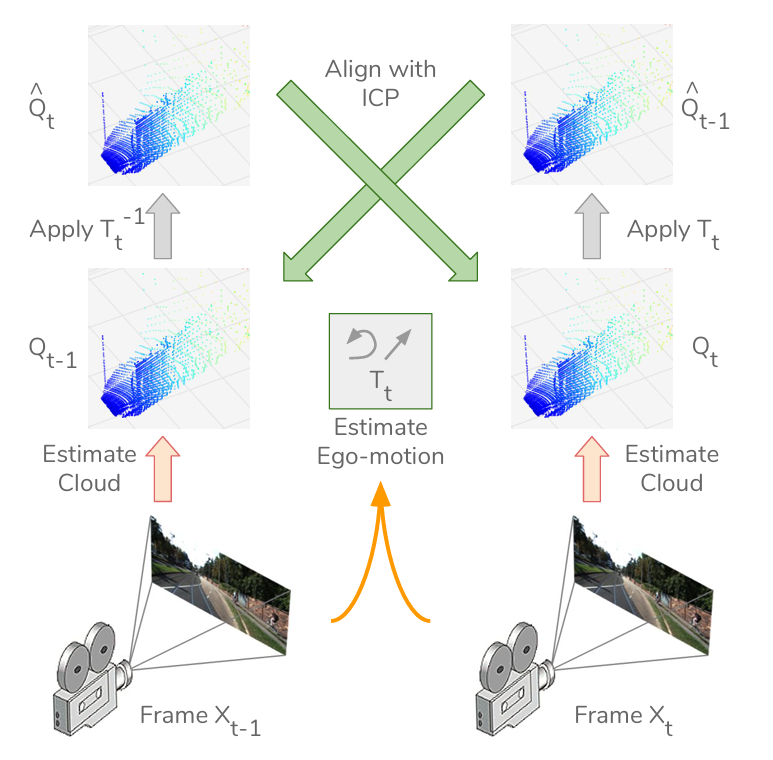
\includegraphics[scale=0.3]{figs/vid2depth}
	\caption{Mahjourian et al. self supervised training pipeline \cite{vid2depth}. \label{fig:vid2depth}}
\end{figure}

The authors' idea is to explicitly constrain consistency on 3D point clouds.
Given two subsequent video frames $\mathbf{I}$ and $\mathbf{J}$, the ego-motion $\mathcal{T} = f_{pose}(\mathbf{I}, \mathbf{J})$ and depth maps of both frames $\mathbf{D}^{\mathbf{I}} = f_{depth}(\mathbf{I}), \mathbf{D}^{\mathbf{J}} = f_{depth}(\mathbf{J})$ are estimated.
Thanks to the (supposedly known) camera intrinsics matrix $\mathbf{K}$, depth maps can be converted into 3D point clouds $\mathbf{Q}_{\mathbf{I}}, \mathbf{Q}_{\mathbf{J}}$.
If $\mathcal{T}$ is the transformation of the camera from $\mathbf{I}$ to $\mathbf{J}$, then $\mathcal{T} ( \mathbf{Q}_{\mathbf{J}} )$ is $\mathbf{Q}_{\mathbf{J}}$ looked from the $\mathbf{I}$ camera and, in theory, it should be identical to $\mathbf{Q}_{\mathbf{I}}$.
A measure of the misalignment of the two point clouds is not defined and, even if it was, it would probably be not differentiable.
Mahjourian et al. solution is to use some registration algorithm for estimating what's the best alignment of the two point clouds by rigid transforming $\mathbf{Q}_{\mathbf{J}}$ to match $\mathbf{Q}_{\mathbf{I}}$ and what the residual error would be.
Then, push $\mathcal{T}$ to match that best rigid transform and push 3D points pair chosen by the algorithm to get more close after the transformation.
They use Iterative Closest Point (ICP) algorithm, which is a registration algorithm that basically tells which points correspond between the two clouds and what's the overall best rigid transformation that one point cloud (following the previous discussion this would be $\mathbf{Q}_{\mathbf{J}}$) should undergo to match the other one($\mathbf{Q}_{\mathbf{I}}$).
"Best" here means that it minimizes the mean distance between the selected point pairs.
So, ICT returns this estimated transform $\hat{\mathcal{T}}$, which can be expressed using its 6 free parameters $(\hat{\theta}_{x}, \hat{\theta}_{y}, \hat{\theta}_{z}, \hat{t}_{x}, \hat{t}_{y}, \hat{t}_{z})$, and directly compared with the ones from the pose-network.
The resulting loss looks like this:
\[
	\big| \hat{\theta}_{x} - \theta_{x} \big| +
	\big| \hat{\theta}_{y} - \theta_{y} \big| +
	\big| \hat{\theta}_{z} - \theta_{z} \big| +
	\big| \hat{t}_{x} - t_{x} \big| +
	\big| \hat{t}_{y} - t_{y} \big| +
	\big| \hat{t}_{z} - t_{z} \big|
\]
This sorts out the pose network optimization, for the depth network it is instead optimized:
\[
	\sum_{p_{\mathbf{I}} \, \text{matches} \, p_{\mathbf{J}}} \big| p_{\mathbf{I}} - \mathcal{T} (p_{\mathbf{Q}}) \big|
\]

%%%%%%%%%%%%%%%%%%%%%%%%%%%%%%%%%%%%%%%%%
%              MonoDepth2
%%%%%%%%%%%%%%%%%%%%%%%%%%%%%%%%%%%%%%%%%
\subsection{MonoDepth2}
Quoting Godard et al. from the abstract of \cite{MonoDepth2}: \textit{"We show that a surprisingly simple model, and associated design choices, lead to superior predictions"}.
In this work they take MonoDepth \cite{MonoDepth} and improve it with clever small tricks without changing the spirit of the method, although adapting it to be trained also on monocular video footage like in \cite{SfMLearner}.
In their edge-aware smoothness loss, the authors substitute $\mathbf{D}$ with its mean normalized value $\mathbf{D} / \text{mean} \mathbf{D}$ to discourage shrinking of the estimated disparity map.
Next they improve the reconstruction error loss: if $\mathbf{I}_{target}$ is reconstructed from $\mathbf{I}_{source, 1}$ obtaining $\hat{\mathbf{I}}_{target, 1}$ and reconstructed from $\mathbf{I}_{source, 2}$ obtaining $\hat{\mathbf{I}}_{target, 2}$, instead of averaging the two reconstruction losses like $\frac{1}{2}(\mathcal{L}_{rec}(\hat{\mathbf{I}}_{target, 1}(p)$, $\mathbf{I}_{target}(p)) + \mathcal{L}_{rec}(\hat{\mathbf{I}}_{target, 2}(p), \mathbf{I}_{target}(p)))$, it is better to minimize the smallest term between the two because the largest is likely linked to phenomenons like occlusion or out-of-view pixel.
Usually if something is occluded in a view, it is not in the other! Same thing for out-of-view pixels.
So it is now minimized
\[
	min \{ \mathcal{L}_{rec}(\hat{\mathbf{I}}_{target, 1}(p), \mathbf{I}_{target}(p)), \, \mathcal{L}_{rec}(\hat{\mathbf{I}}_{target, 2}(p), \mathbf{I}_{target}(p)) \}
\]
Another clever improvement Godard et al. make is to apply an auto-masking procedure for stationary pixels.
Static pixels can correspond to a static camera or to objects moving at the same velocity of the camera.
If a pixel $p$ is such that $\mathcal{L}_{rec}(\mathbf{I}_{target}, \mathbf{I}_{source})(p)$ is "low", then there are three likely alternatives:
\begin{enumerate}
\item the camera is not moving and that pixel corresponds to a static object
\item the camera is moving and that pixel corresponds to an object moving in the same direction and speed of the camera
\item that pixel corresponds to a low texture area, hence, independently of the dynamics of the scene, it is similar across adjacent frames.
\end{enumerate}
The heuristic is to mask out pixels that have this "low" comparison error.
Godard et al. exclude pixels with comparison error smaller than the reconstruction error:
\[
	\text{min}_{source} \{ \mathcal{L}_{rec}(\mathbf{I}_{target}, \mathbf{I}_{source})(p) \}
		\leq
	\text{min}_{source} \{ \mathcal{L}_{rec}(\mathbf{I}_{target}, \hat{\mathbf{I}}_{target})(p) \}
\]
Taking the minimum is done also here for the same reasons explained above.
Their observations and tricks continue on the architectural side.
For instance, they up-sample the lower resolution depth maps returned by their multiscale network instead of decreasing the resolution of the ground truth data during training.
They also apply reflection padding to input images to decrease border artifacts, as opposed to zero-padding.

%%%%%%%%%%%%%%%%%%%%%%%%%%%%%%%%%%%%%%%%%
%              struct2depth
%%%%%%%%%%%%%%%%%%%%%%%%%%%%%%%%%%%%%%%%%
\subsection{struct2depth}
What's the next step? To weaken assumptions.
One very limiting assumption was that video footage scenes were static, i.e. nothing moves.
In \cite{struct2depth} Casser et al. try to include the motion of the objects into their framework, which they call struct2depth (see figure \ref{fig:struct2depth}).
They are not the first to model dynamic scenes for improving depth estimation from subsequent frames, but they are the first that model individual objects movements rather than using 2D or 3D optical flow.

% architecture
\begin{figure}
	\centering
	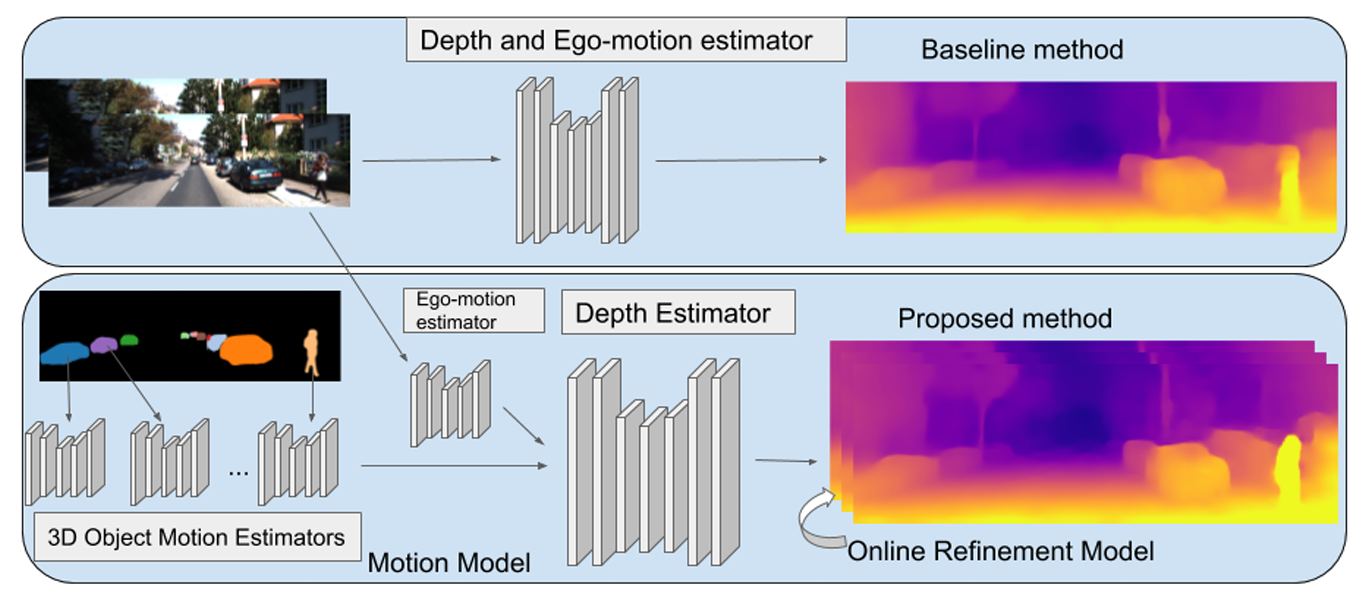
\includegraphics[scale=0.3]{figs/struct2depth}
	\caption{Casser et al. struct2depth \cite{struct2depth} model. \label{fig:struct2depth}}
\end{figure}

As always let's first simplify the approach.
Consider an object which appears in subsequent frames, if images are masked so that only the object is visible, the relative transformation of the camera w.r.t. it can be estimated.
Thanks to that it might be reconstructed the object appearance in one frame from its appearance in the other.
More precisely, consider $\mathbf{I}_{0}$ and $\mathbf{I}_{1}$ are the two frames and the object masks are $\mathbf{O}_{0}$ and $\mathbf{O}_{1}$ (which can be computed by means of a given instance-aligned segmentation model $f_{segment}$).
The relative camera transformation $\mathcal{T}$ can be estimated as $f_{pose}(\mathbf{I}_{0} \odot \mathbf{O}_{0}, \, \mathbf{I}_{1} \odot \mathbf{O}_{1})$, with $\odot$ representing pixel-wise multiplication.
For reconstruction purpose, a depth map is estimated from the first image: $\mathbf{Z}_{0} = f_{depth}(\mathbf{I}_{0})$.
Now $\mathbf{Z}_{0}$ gives the depth of the object in the nonzero pixels of its mask $\mathbf{O}_{0}$.
The same reconstruction of the previous methods is applied.
The only difference is not all target image $\mathbf{I}_{1}$ pixels are filled, but just the ones corresponding to the object, i.e. the non-masked pixels from $\mathbf{O}_{1}$.

The way the authors put all of this together in an actual procedure is a bit more complicated, here only a general overview is reported.
They consider three frames and target the middle one for the reconstruction by first applying the illustrated procedure on the background mask and actually reconstructing the whole image without considering moving objects artifacts.
Then they segment the objects in this reconstruction and apply the procedure again to them.
In this way they separate objects motion from ego-motion and for this purpose they use two different pose networks.
For technical details and considerations they follow along Godard et al. and their MonoDepth2 \cite{MonoDepth2}.

One important contribution of Casser et al. work is to include constraints on object sizes in regressing the depth.
This is very clever and solves a problem encountered in MonoDepth2 which was there tackled using stereo data.
If I am in a car capturing video footage and in front of me there is a car moving at the same speed, the model will assign to it "infinite" depth, like it were a very far background detail like the sky is.
For solving this, Casser et al. guess the depth of the objects based on their size (i.e. area) and class (car, tree, person, ...) and constrain also the depth model to have a similar guess.

There are other things that could be added, but I think this is sufficient to grasp the general concept.

%%%%%%%%%%%%%%%%%%%%%%%%%%%%%%%%%%%%%%%%%
%              struct2depth
%%%%%%%%%%%%%%%%%%%%%%%%%%%%%%%%%%%%%%%%%
\subsection{FeatDepth}
Why need I compare images using their appearance and not some higher representation of them?
No reasons, in fact Shu et al. \cite{FeatDepth} propose to compare reconstructed images based on their feature maps.

% training pipeline
\begin{figure}
	\centering
	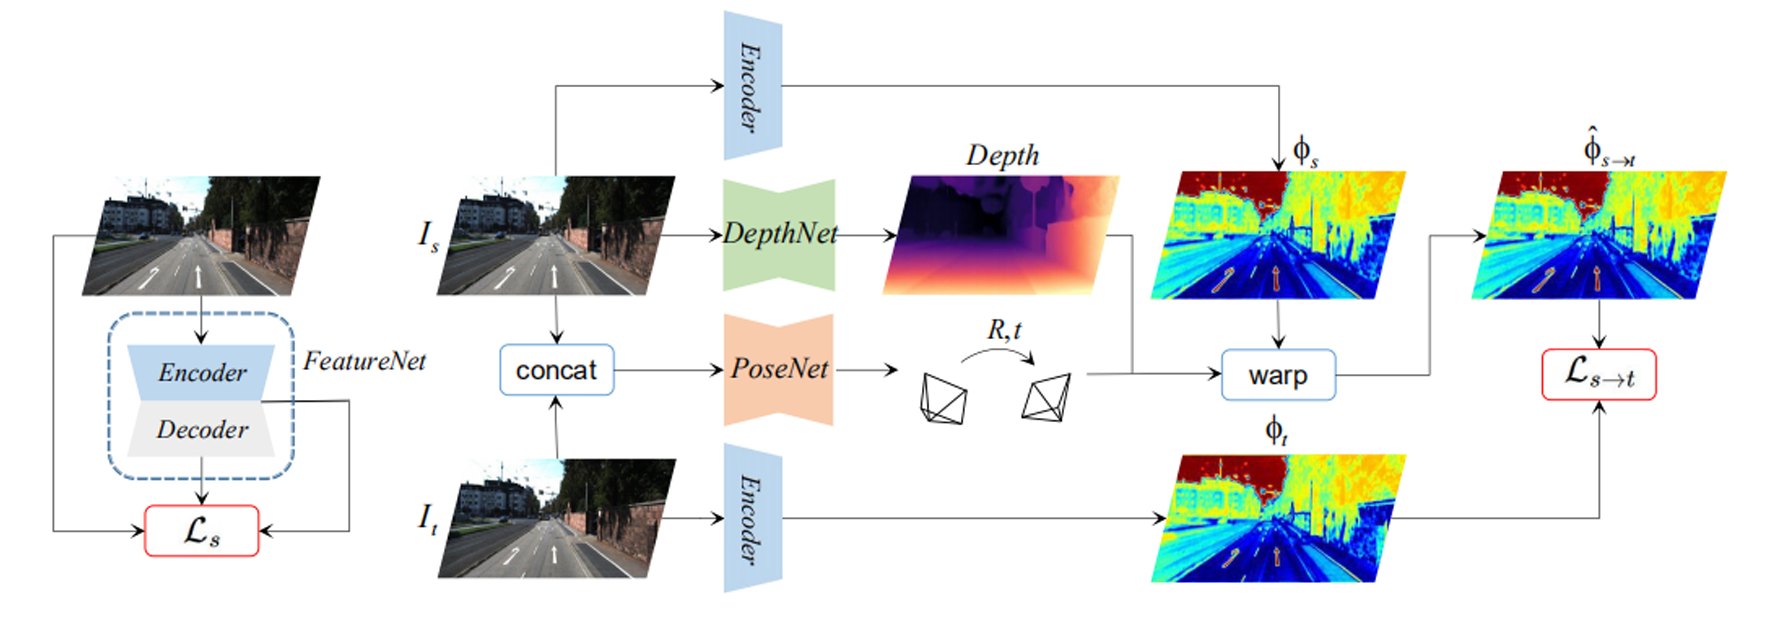
\includegraphics[scale=0.3]{figs/featdepth}
	\caption{Shu et al. FeatDepth \cite{FeatDepth} pipeline. Note that the image is taken from the paper and uses a different notation. \label{fig:featdepth}}
\end{figure}

They argue that correct depth and pose are sufficient but not necessary for small photometric error.
The cause of this is texture-less regions which produce low photometric error even with wrong depth and pose estimates.
The authors' idea is then to use some higher representation of the image encouraging it to be discriminative also where the image is not.
For achieving this, Shu et al. employ three networks: DepthNet and PoseNet, as in the previous works, and FeatureNet which is an encoder based on ResNet-50 \cite{ResNet}.
If $\mathbf{F}$ is the deep multi-channel feature map of the image to reconstruct $\mathbf{I}$ and $\mathbf{F}_{rec}$ the one of the reconstructed image $\mathbf{I}_{rec}$, then the following losses are used:
\[
	\mathcal{L}_{rec} = \text{mean}_{p \in \mathbf{F}} \big\| \mathbf{F}(p) - \mathbf{F}_{rec}(p) \big\|_{1}
\] \[
	\mathcal{L}_{dis} = - \text{mean}_{p \in \mathbf{F}} \big\| \nabla^{1} \mathbf{F}(p) \big\|
\] \[
	\mathcal{L}_{cvt} = \text{mean}_{p \in \mathbf{F}} \big\| \nabla^{2} \mathbf{F}(p) \big\|
\]
$\mathcal{L}_{rec}$ is the reconstruction error measured in the feature space.
$\mathcal{L}_{dis}$ encourages the learned feature maps to have gradients, making also texture-less regions well characterized.
Lastly, $\mathcal{L}_{cvt}$ is a regularization term favouring the convergence of the method.

The architecture of FeatDepth is improved in GCNDepth \cite{GCNDepth} by other authors.
They use a Graph Convolutional Network (GCN) for mapping intermediate decoder feature maps to depth maps.
They manage to reduce the size of their model of 40\% w.r.t. the FeatDepth.

%\section{SOTA}

%%%%%%%%%%%%%%%%%%%%%%%%%%%%%%%%%%%%%%%%%
%              MiDas
%%%%%%%%%%%%%%%%%%%%%%%%%%%%%%%%%%%%%%%%%
All the methods introduced suffer from poor generalization and poor transferability to other datasets and to unconstrained scenes.
In fact the main depth estimation datasets are not sufficiently rich to train a robust model.
The advancement that makes a leap forward is MiDas \cite{MiDas}, which stands for "Mixing Datasets".
MiDas is a technique for training a depth estimation model on diverse labeled data by using a loss function that is invariant to the various differences among datasets.
The authors of \cite{MiDas} also used 3D-movies as source of stereo data and they did a great work in cleaning it up and converting it to suitable disparity maps.
Three main incompatibilities arise across different datasets:
\begin{enumerate}
	\item Ground truth representation, which can be a depth map or a disparity map
	\item Scale ambiguity, some datasets use relative depth and others provide up-to-scale depth maps
	\item Shift ambiguity, in particular in 3D movies stereo pairs present a global disparity shift.
\end{enumerate}
First: they choose to work in disparity space.
Then, when comparing a ground truth disparity map $\mathbf{d}_{gt}$ and a predicted disparity map $\mathbf{d}_{pred}$ they scale and shift the two so that they have zero shift and unit scale.
They approximate the idea of "scale" and "shift" by means of two functions $s$ and $t$:
\[
	t(\mathbf{d}) := \mathop{\text{median}}_{p \in \mathbf{d}}(\mathbf{d}(p))
\] \[
	s(\mathbf{d}) := \mathop{\text{mean}}_{p \in \mathbf{d}} \big| \mathbf{d}(p) - t(\mathbf{d}) \big|
\] \[
	\hat{\mathbf{d}}_{pred} = \frac{\mathbf{d}_{pred} - t(\mathbf{d}_{pred})}{s(\mathbf{d}_{pred})}
\] \[
	\hat{\mathbf{d}}_{gt} = \frac{\mathbf{d}_{gt} - t(\mathbf{d}_{gt})}{s(\mathbf{d}_{gt})}
\]
Finally their scale and shift invariant($ssi$) loss is:
\[
	\mathcal{L}_{ssi} = \mathop{\text{mean}}_{p \in \mathbf{d}} \big| \hat{\mathbf{d}}_{pred}(p) - \hat{\mathbf{d}}_{gt}(p)\big|
\]
They regularize it using the following term, which biases the prediction discontinuities to match the ones in the respective ground truth:
\[
	\mathcal{L}_{reg} = \mathop{\text{mean}}_{p \in \mathbf{d}}
		\left(
			\big| \partial_{x} (\hat{\mathbf{d}}_{pred} - \hat{\mathbf{d}}_{gt}) \big| +
			\big| \partial_{y} (\hat{\mathbf{d}}_{pred} - \hat{\mathbf{d}}_{gt}) \big| 
		\right)(p)
\]
Lastly they discuss the mixing strategies for sampling the datasets in the mini-batches of the stochastic gradient descent algorithm.
They propose to use a Pareto-optimal strategy from \cite{pareto}, this mixing-strategy will be used in many subsequent works while the loss they introduced is often replaced by the scale-invariant loss from \cite{Eigen}.
They use some datasets for training and some for testing, using the experimental protocol called \textit{zero-shot cross-dataset transfer}.
The model architecture is an encoder-decoder-like model as in \cite{ReDWeb}. Their full work and code can be found at \url{https://github.com/isl-org/MiDaS}, here the matter has been simplified for brevity.

%%%%%%%%%%%%%%%%%%%%%%%%%%%%%%%%%%%%%%%%%
%              PatchFusion
%%%%%%%%%%%%%%%%%%%%%%%%%%%%%%%%%%%%%%%%%
Li et al. \cite{PatchFusion} address the problem of metric monocular depth estimation for high-resolution inputs.
Their method, PatchFusion, aligns with so called \textit{Tile-Based Methods}.

% architecture
\begin{figure}
	\centering
	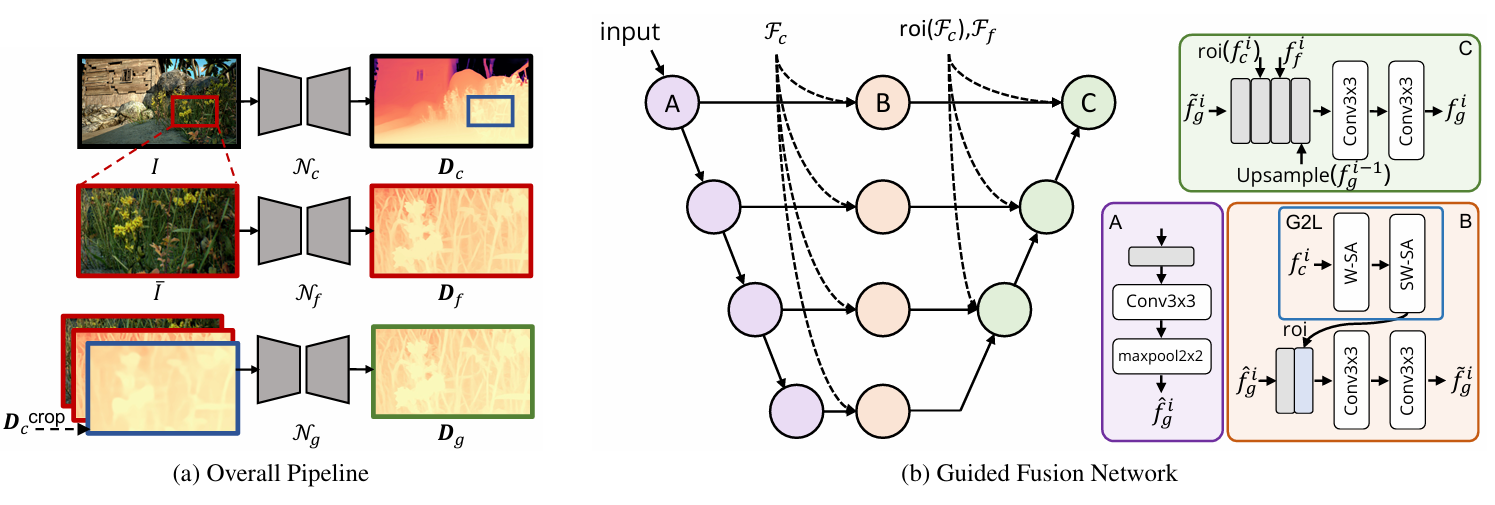
\includegraphics[scale=0.3]{figs/patchfusion}
	\caption{Li et al. architecture \cite{PatchFusion}. \label{fig:patchfusion}}
\end{figure}

The architecture employed is composed of three networks: a global-scale aware prediction network which takes as input a high-resolution down-sampled image and outputs a coarse depth map; a patch-wise depth prediction network which takes as input an image patch and outputs its fine relative depth map; a guided-fusion network.
The guided-fusion network is intricate, but its role is to further process the fine depth map of a patch to make it scale-aware.
It takes as inputs the fine depth map and the corresponding patches in the original image and in the coarse depth map.
With this machinery is now possible to divide a high-resolution image in patches and compute a depth map for each patch, obtaining a depth map for the whole image, but patch artifacts are yet to be removed.
To this end \textit{Consistency-Aware Training} is performed by subdividing the images in overlapping patches and minimizing also the agreement between the patch depth maps and feature maps.
If $\rho_{1}$ and $\rho_{2}$ are two overlapping patch depth maps and $\phi_{1}$, $\phi_{2}$ their respective feature maps, the consistency-aware loss term is:
\[
	\mathcal{L}_{consistency} = \mathop{\text{mean}}_{p \in \phi_{1} \cap \phi_{2}} \left( \big\| \phi_{1}(p) - \phi_{2}(p) \big\|_{2} + \mu \big| \rho_{1}(p) - \rho_{2}(p) \big| \right)
\]
Where $\mu$ is, with no surprises, a hyperparameter.
One important technical detail of their guided-fusion network is that SwinTransformer layers \cite{swin} are used to process feature maps and preserve global context \cite{PatchFusion}.
Code and everything at \url{https://zhyever.github.io/patchfusion/}.\\
\\
Ke et al. \cite{Marigold} prove that a comprehensive representation of the visual world is the cornerstone of (relative) monocular depth estimation.
Their insight is to use priors learned by generative diffusion models to enable more generalizable depth estimation, in particular they adopt Stable Diffusion v2 \cite{StableDiffusionV2} pretrained Variational Auto Encoder(VAE) and Latent Diffusion U-Net.
Monocular depth estimation is here posed as a conditional denoising diffusion generation task.
The idea is to teach a model called "diffusion model" to clean a depth map from noise conditioned to the corresponding RGB image.
More formally consider an RGB image $I$, its depth map $\rho$ and its noise corrupted depth map $\tilde{\rho}_{0}$ (which can be so corrupted to be just sampled random noise, i.e. $\rho$ needn't be known), the diffusion model takes as input the two and outputs a less noisy depth map $\tilde{\rho}_{1}$.
The noise is modeled as additive, hence $\tilde{\rho}_{1} = \tilde{\rho}_{0} + \epsilon(I, \tilde{\rho}_{0})$, where $\epsilon$ is the computed noise to remove.
After repeating the procedure a few times the resulting depth map is expected to match the ground truth depth map: $\tilde{\rho}_{T} \approx \rho$.
Actually, all this process takes place in a \textit{latent space}, meaning that instead of working with depth maps and images, the diffusion model works with their lower dimensional representations computed by the encoder $\mathcal{E}$ from the pretrained Stable Diffusion VAE(and with fixed parameters) and noise is added in that space.
For getting the final depth estimate the decoder $\mathcal{D}$ from the same VAE is used.
I'm not giving all the details here, but one thing to know is how a pretrained model that works with RGB images can work with depth maps: depth maps are first affinely trasformed to be in approximately the range $[-1, +1]$ and then are replicated into three channels.
In this way they are compatible with the Stable Diffusion VAE.
Nevertheless, it is not obvious at all that the VAE can reconstruct this kind of image, but Ke et al. experimentally observed that $\rho \approx \mathcal{D}(\mathcal{E}(\rho))$ with a negligible error.
This is quite surprising to me.
Another remarkable fact is that Marigold is trained only on synthetic data and generalizes so well to real world data that beats various other methods in almost every unseen test dataset they evaluated the model on. Ke et al. definetily proved their point.
Here the link to their work \url{https://marigoldmonodepth.github.io/}.
%-------------------------------------------------------------------
\chapter{Tools and Frameworks}
\label{c:tools}
%-------------------------------------------------------------------

\epigraph{\enquote{I believe that inside every tool is a hammer.}}{\emph{Adam Savage}}

This chapter describes the tools and frameworks used in the thesis.

%-------------------------------------------------------------------
\chapter{Implementation}
\label{c:implementation}
%-------------------------------------------------------------------

\epigraph{\enquote{Sometimes, the elegant implementation is just a function. Not a method. Not a class. Not a framework. Just a function.}}{\emph{John Carmack}}

This capter shows the details of the implementation of the work.

%-------------------------------------------------------------------
\chapter{Results}
\label{ch:results}
%-------------------------------------------------------------------

\epigraph{\enquote{All models are wrong, but some are useful.}}{\emph{George Box}}

This chapter shows and discusses the results obtained in the thesis.
%In section \ref{sec:experiments} the experimental setting is described and numerical results are reported.
%In section

\section{Experiments}
\label{sec:experiments}

\paragraph{Architecture.}
A neural network model was trained to predict \textit{metric} depth values on image patches.
The neural architecture used is the one from~\cite{Eigen}, with some modification.
Instead of treating it as a two-stage architecture with a component estimating a coarse depth map and another one refining it, it was treated as an end-to-end method.
The network is illustrated in figure~\ref{fig:Eigen}, its backbone is a pretrained AlexNet.
The input image normalization was also modified.
The normalization applied shifts image input values from $[0, 1]$ to $[-1, 1]$.
Finally, an adaptive average pooling layer reduces the deeper feature map of the convolutional part of AlexNet to a feature vector of size 4096.

This model has to be considered a toy model since it is based on the first deep learning architecture ever used for DE (2014).
As later graphs will show, its learning capabilities are limited.

\paragraph{Training.}
The dataset used is KITTI~\cite{KITTI} with the Eigen split, that is the subdivision of the KITTI dataset into train, validation and test subsets originally used by Eigen~et~al. in~\cite{Eigen} and used as a benchmark from there on.
Depth maps are built directly from 3D point clouds, a simplification was performed in this phase to make the code signficantly faster.
This simplification introduces inaccuracies.
But, since training the model like Eigen~et~al. showed only little degradation in metric scores (attributable also the changing on the architectural side), the modification was kept.

The model obtained as input image patches of size fixed to $150 \times 150$.
From each image a batch of 8 patches was extracted.
Two extraction methods were tried: random sampling patches and sampling patches centered in some detected corner.
Patches were further processed before prediction.
It was experimented with geometrical correction of distorsions introduced by the camera far from its principal point.
So experiments were performed either with warping or without it.
After this optional transformation, three options were tried: leave the patch as it is, radially blurring it, uniformly blurring it.

In total there are three options: sampling strategy (random vs corner), patch warping (warp vs no warp), blurring (no blur vs radial blur vs uniform blur).
These result in 12 experiments.

Each experiment consisted in a training of 4 epochs and a stochastic gradient descent optimizer with learning rate 0.0001 and momentum 0.9.
An L1 regularization to the network weights (multiplied by 0.01) was applied for making the algorithm more numerically stable.

The loss function was common to each experiment and is a radially weighted scale invariant loss.
It is a modification of the loss from Eigen~et~al.~\cite{Eigen}.
Their loss is defined in section~\ref{sec:regression_methods}.
Each pixel contribution to the loss is weighted with a gaussian density function with $\sigma = (h + w) / 2$ evaluated in the distance of the pixel from the center of the patch.

\paragraph{Validation.}
Figures \ref{fig:validation} and \ref{fig:Wvalidation} show metrics measured during validation phase.
Both the metrics discussed in section~\ref{sec:metrics} and defined in table~\ref{t:metrics} and their weighted counterparts are shown.
It can be observed that validation performance saturates and sometimes also degrades on the fourth epoch.
This shows that the model learning capabilities are fairly limited as it quickly stops improving itself.
This was expected since the model is old and has known limitations like the fully-connected layers used for up-sampling the feature maps to a depth prediction.
While fully-connected layers proved successful in various tasks, other solutions showed to be more useful in computer vision, as the history of this field proves.

\begin{figure}
    \begin{adjustwidth}{-0.2\textwidth}{-0.2\textwidth}
    \centering
        \begin{subfigure}{0.6\textwidth}
            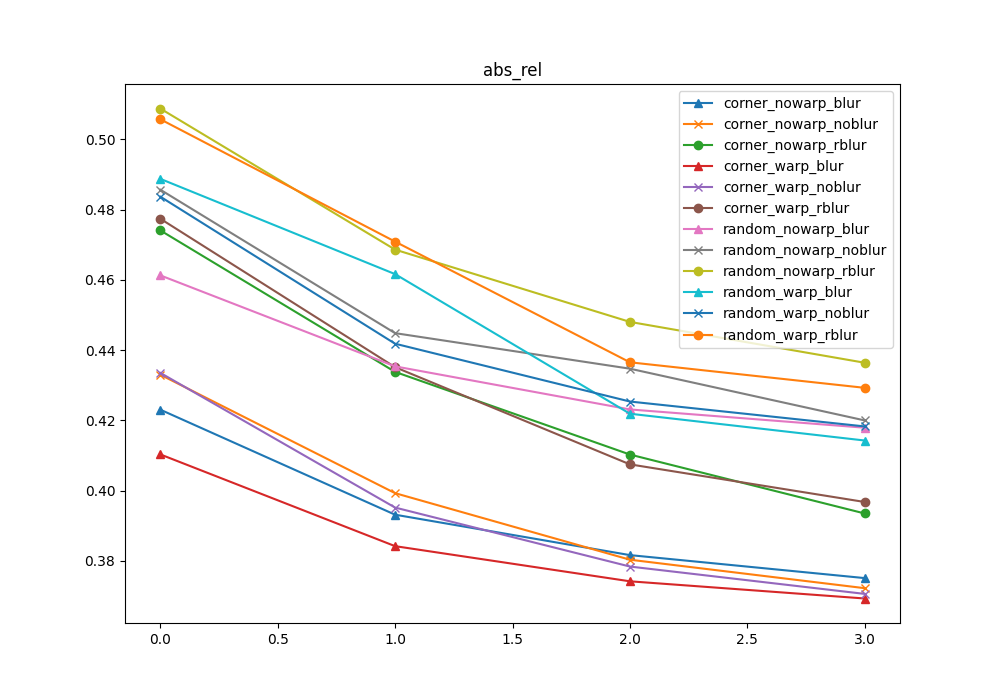
\includegraphics[width=\textwidth]{figs/abs_rel}
        \end{subfigure}
        \hspace{0cm}
        \begin{subfigure}{0.6\textwidth}
            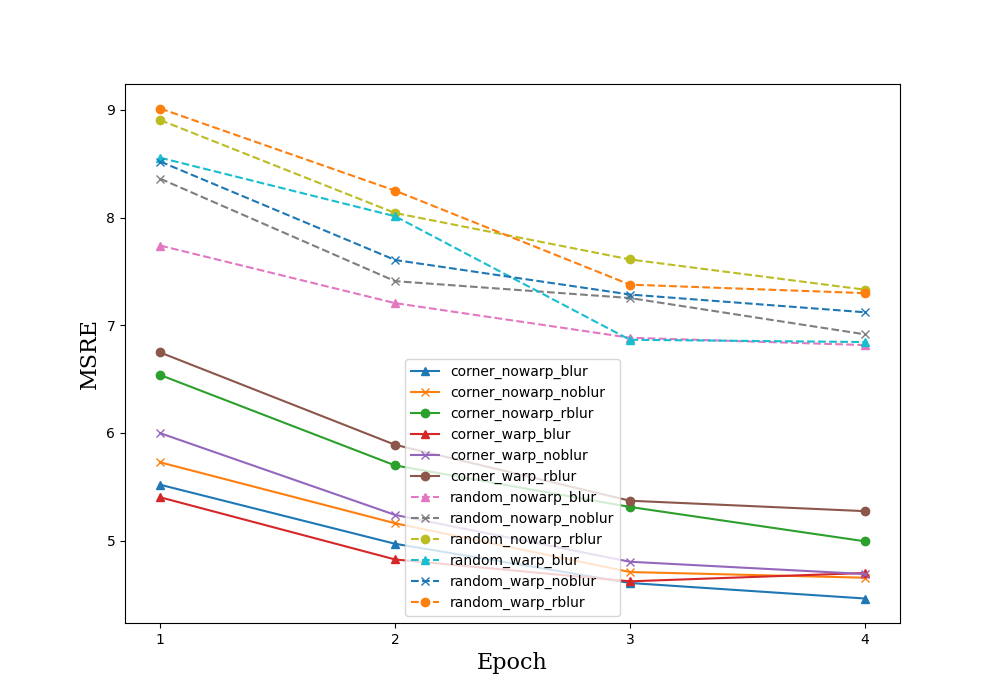
\includegraphics[width=\textwidth]{figs/sq_rel}
        \end{subfigure}
        \hspace{0cm}

        \begin{subfigure}{0.6\textwidth}
            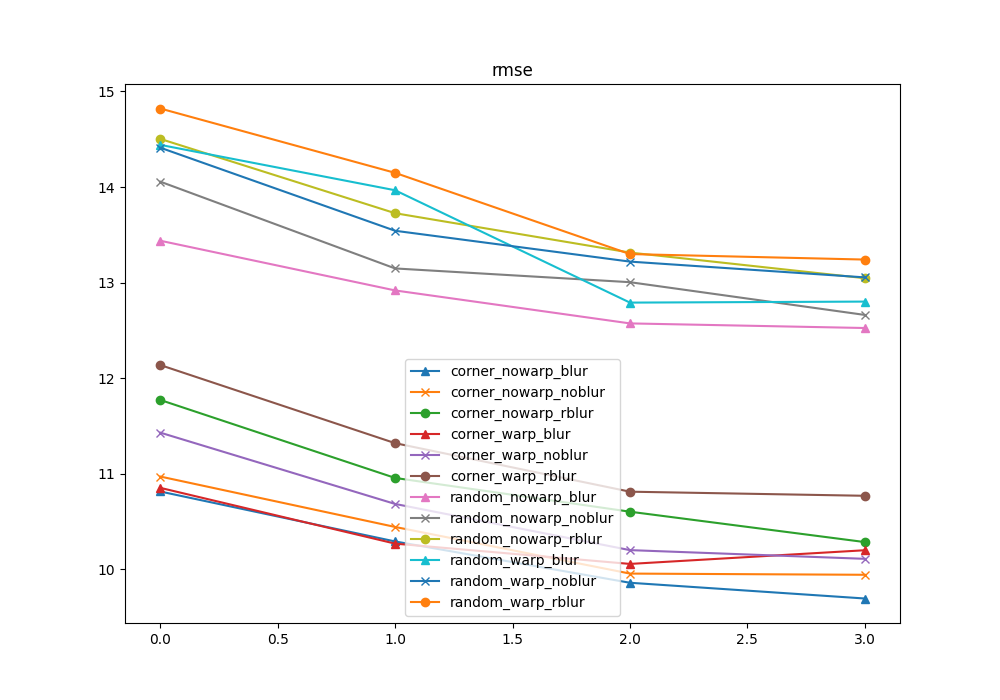
\includegraphics[width=\textwidth]{figs/rmse}
        \end{subfigure}
        \hspace{0cm}
        \begin{subfigure}{0.6\textwidth}
            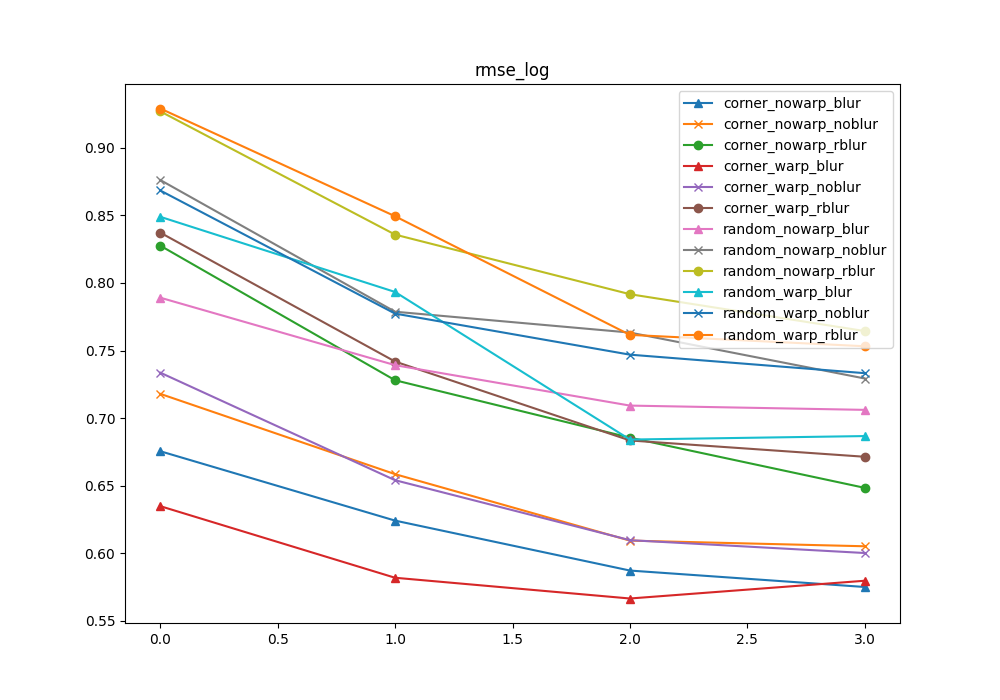
\includegraphics[width=\textwidth]{figs/rmse_log}
        \end{subfigure}
        \hspace{0cm}
        \begin{subfigure}{0.6\textwidth}
            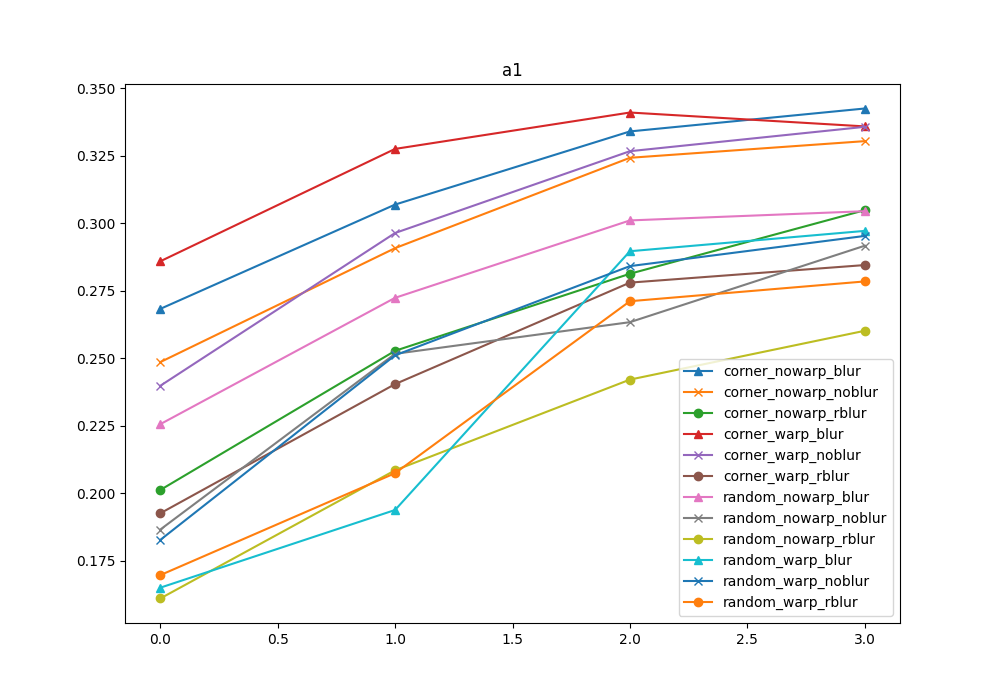
\includegraphics[width=\textwidth]{figs/a1}
        \end{subfigure}
        \hspace{0cm}
        \begin{subfigure}{0.6\textwidth}
            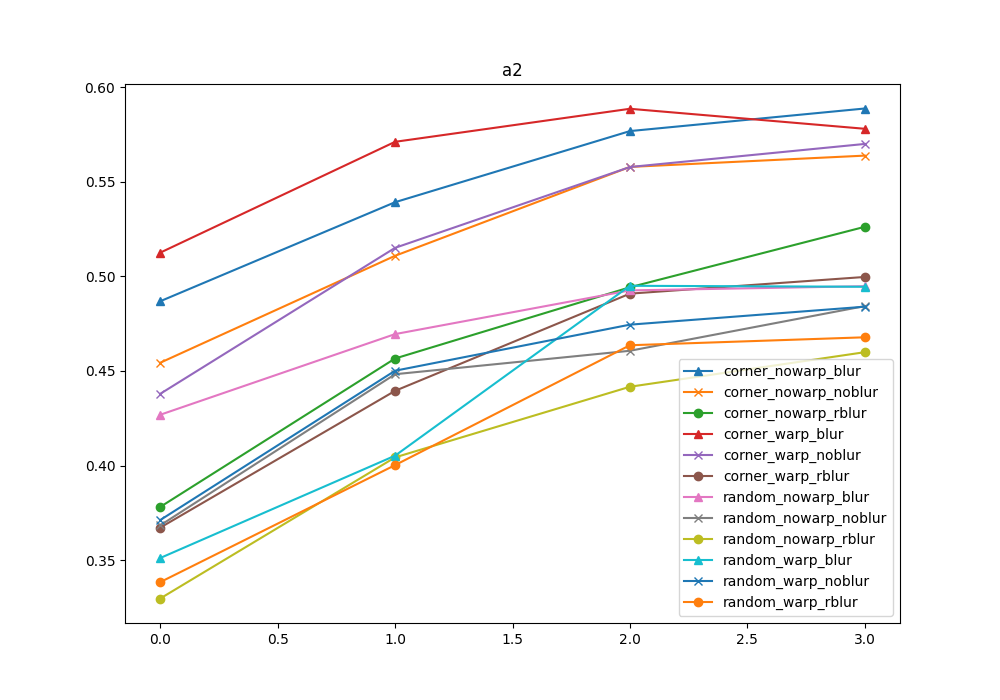
\includegraphics[width=\textwidth]{figs/a2}
        \end{subfigure}
        \hspace{0cm}

        \begin{subfigure}{0.6\textwidth}
            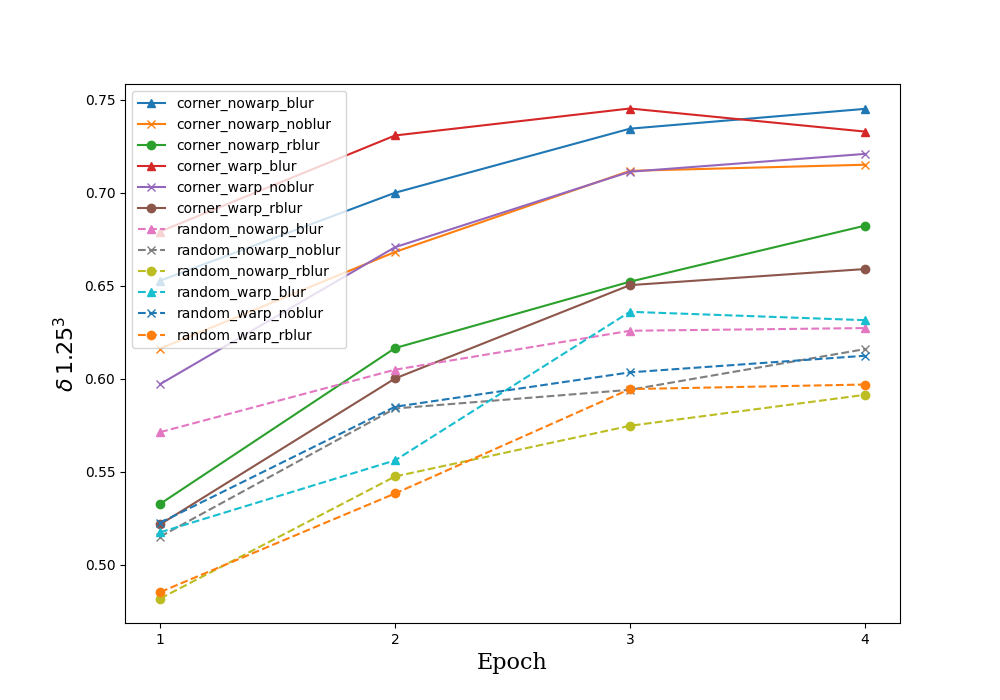
\includegraphics[width=\textwidth]{figs/a3}
        \end{subfigure}
    \end{adjustwidth}
    \caption{
        Non-weighted metrics computed during the validation phase.
        \label{fig:validation}
    }
\end{figure}

\begin{figure}
    \begin{adjustwidth}{-0.2\textwidth}{-0.2\textwidth}
    \centering
        \begin{subfigure}{0.6\textwidth}
            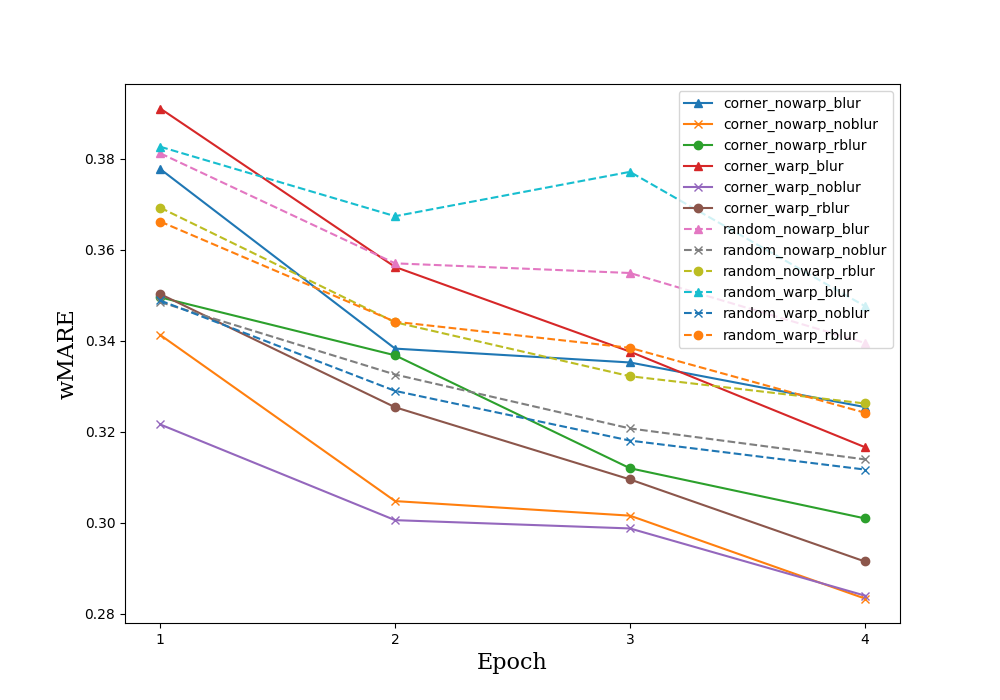
\includegraphics[width=\textwidth]{figs/wabs_rel}
        \end{subfigure}
        \hspace{0cm}
        \begin{subfigure}{0.6\textwidth}
            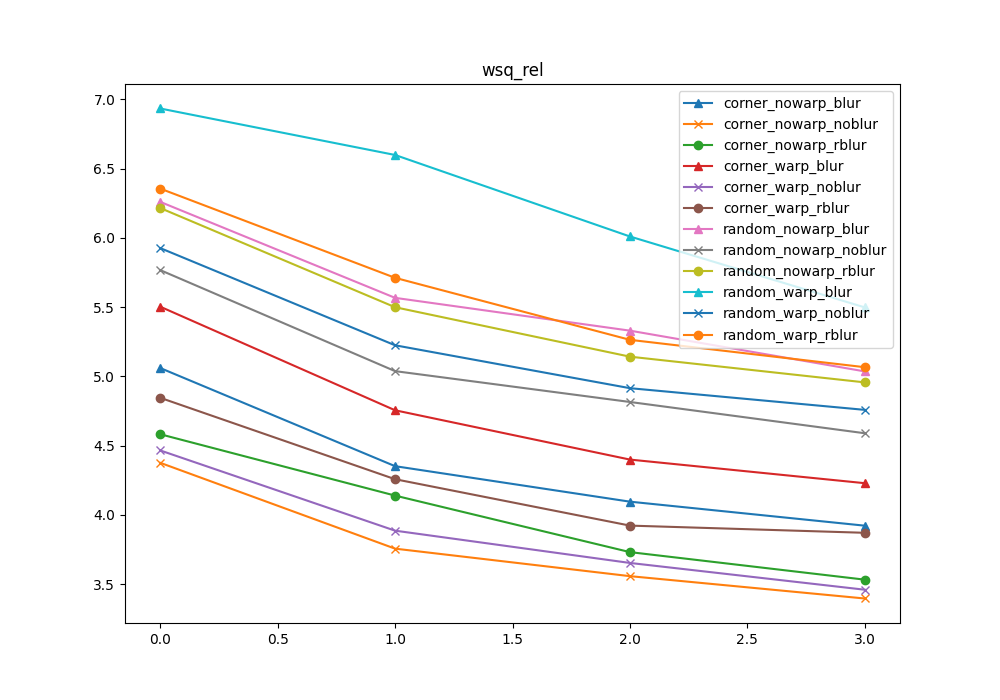
\includegraphics[width=\textwidth]{figs/wsq_rel}
        \end{subfigure}
        \hspace{0cm}

        \begin{subfigure}{0.6\textwidth}
            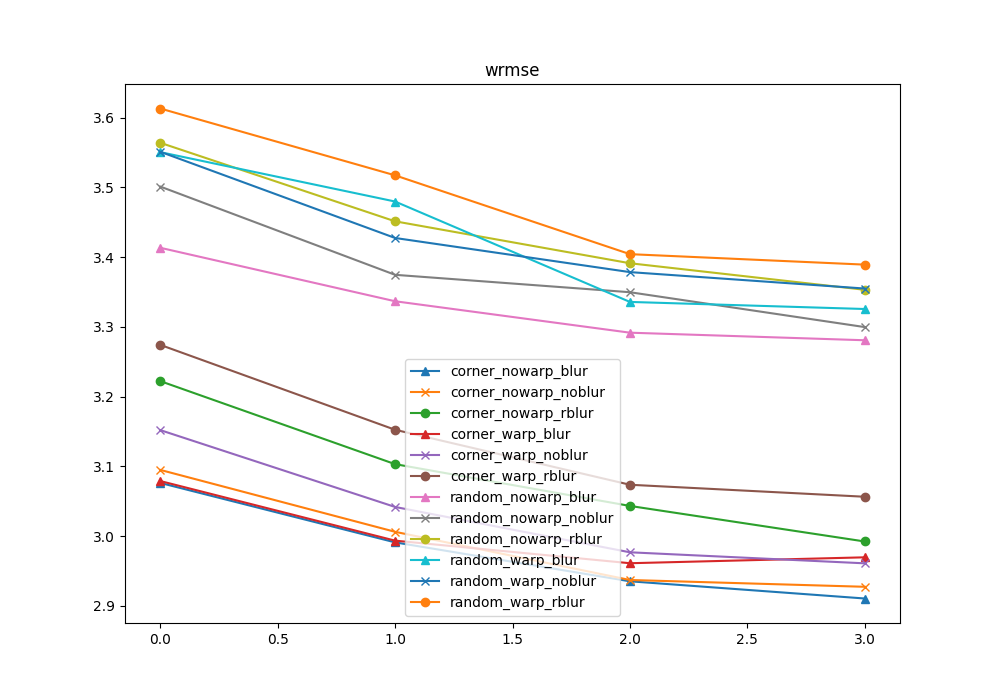
\includegraphics[width=\textwidth]{figs/wrmse}
        \end{subfigure}
        \hspace{0cm}
        \begin{subfigure}{0.6\textwidth}
            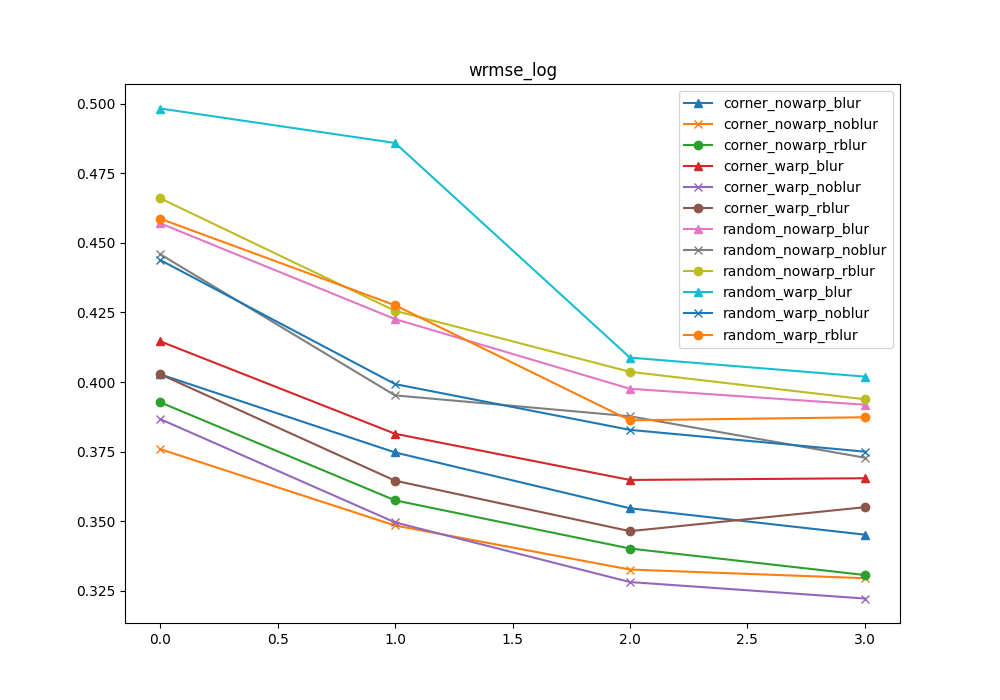
\includegraphics[width=\textwidth]{figs/wrmse_log}
        \end{subfigure}
        \hspace{0cm}
        \begin{subfigure}{0.6\textwidth}
            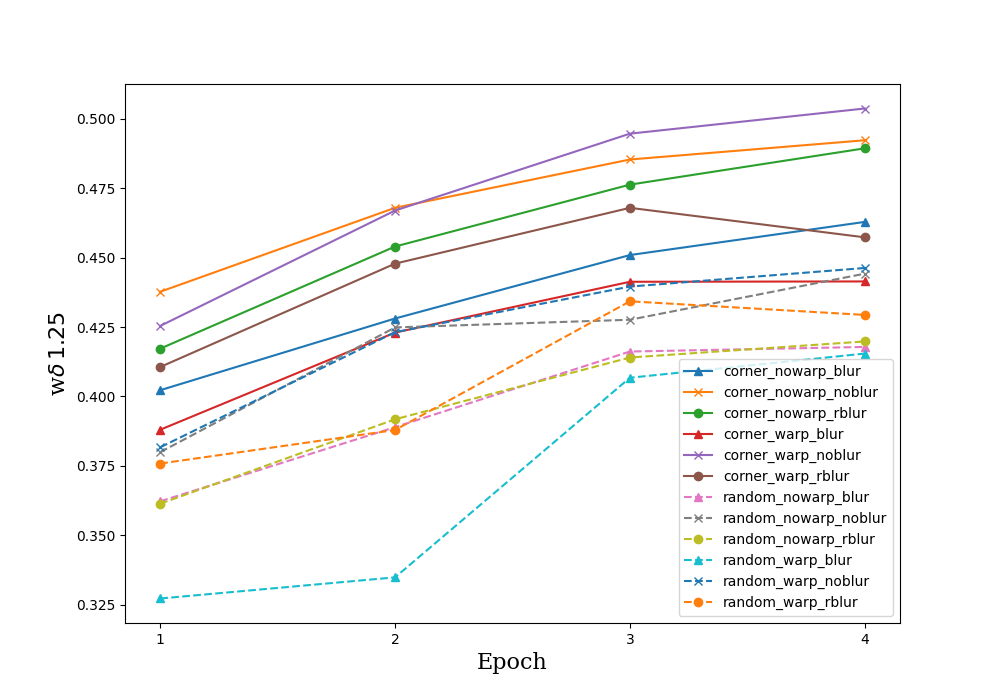
\includegraphics[width=\textwidth]{figs/wa1}
        \end{subfigure}
        \hspace{0cm}
        \begin{subfigure}{0.6\textwidth}
            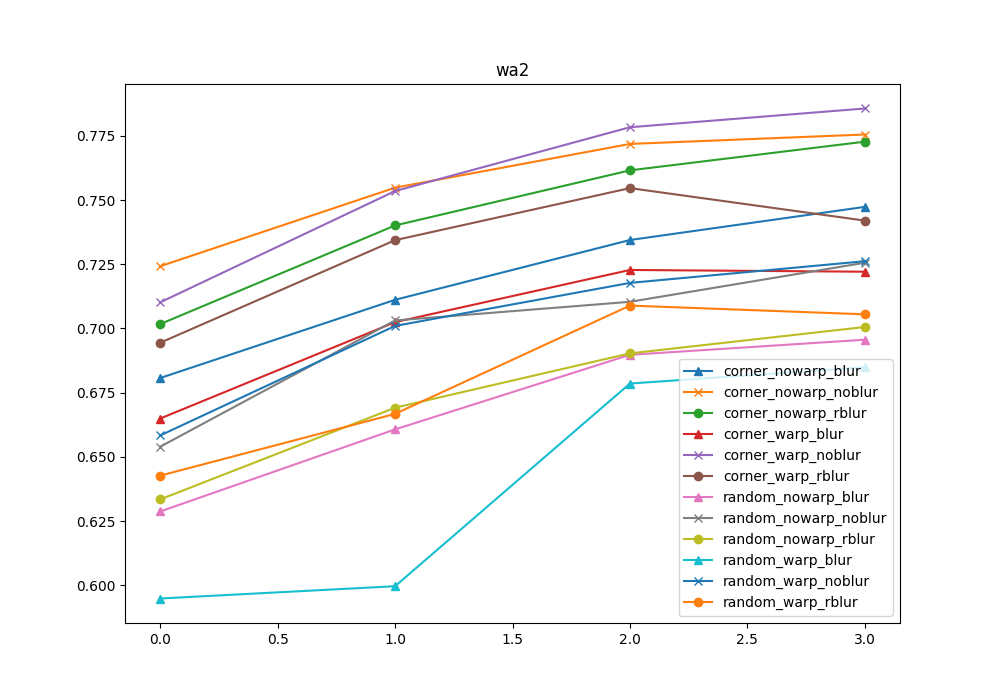
\includegraphics[width=\textwidth]{figs/wa2}
        \end{subfigure}
        \hspace{0cm}

        \begin{subfigure}{0.6\textwidth}
            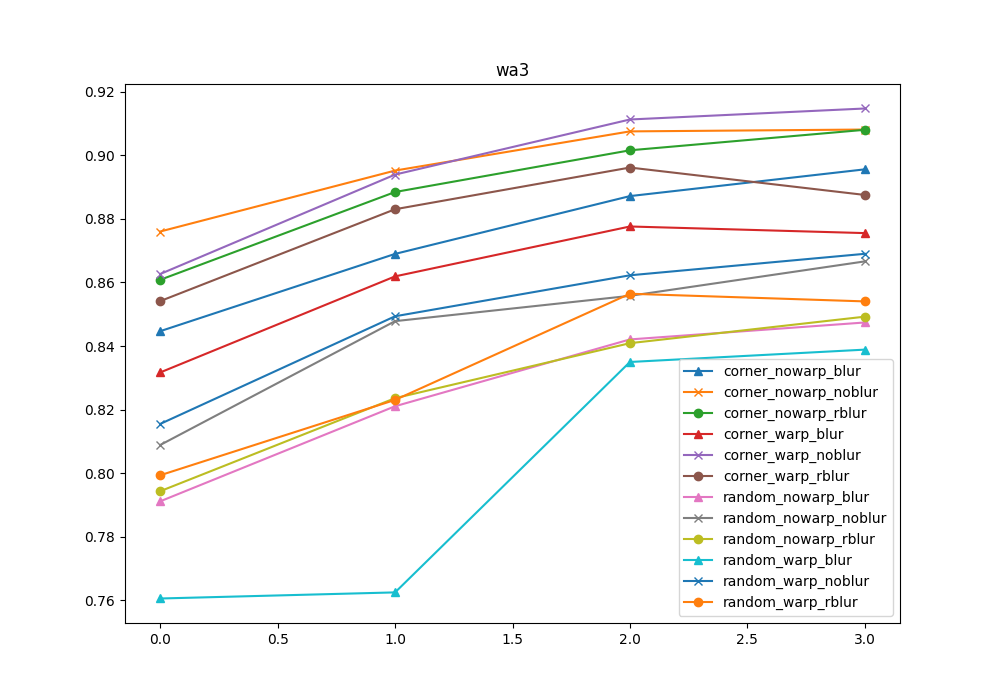
\includegraphics[width=\textwidth]{figs/wa3}
        \end{subfigure}
    \end{adjustwidth}
    \caption{
        \textbf{Weighted} metrics computed during the validation phase.
        \label{fig:Wvalidation}
    }
\end{figure}

\section{Discussion}
\label{sec:discussion}

All the trained models were tested on a held-out subset of the KITTI defined by the Eigen split.
All the numerical results obtained are reported in tables~\ref{t:results} and~\ref{t:weighted_results}.
The effect of each of the three options are now discussed: sampling strategy, warping and blurring.
These options are used both for training and evaluation.
Each of them defines a different learning problem with a different data distribution.
Single image depth estimation (SIDE) can be performed by fusing the predictions produced by each of the proposed learning setups.
To this extent, picking the options that maximize the performances allows for a better overall SIDE.
Results must be interpreted keeping this in mind.

\paragraph{Effect of sampling strategy.}
It is evident that the corner sampling defines a learning problem on which the network performs better.
This was also notable in the validation graphs and is true for all metrics without exceptions.
In~\cite{BoostingDepth} was observed that pretrained SIDE models perform better on image regions with a certain edge density.
Here it is proved that defining the SIDE problem on better-behaved image regions results in a simpler learning problem for the model.
This is likely due to a correlation of corners with visual depth cues.

\paragraph{Effect of warping.}
Warping seems to mildly simplify the learning problem too.
In the non-weighted metrics table~\ref{t:results}, while some best or second-to-best results are associated to the presence of warping, there isn't an overall performance improvement.
Instead, in table~\ref{t:wighted_results}, warping is present in all best performing models except for one problem setting.
Since the training loss was itself weighted, the weighted metrics are the reference for these experiments.
Hence, it can be concluded that: geometrically correcting the patches by appropriately warping them lead to little improvements.
Further investigation is needed for assessing the real utility of this additional preprocessing.
In any case, it must be noted that the warping procedure itself introduces some interpolation error that could have influenced results.
There could be better warping procedures that are less affected by this.

\paragraph{Effect of blurring.}
The radial blurring options never appears in the best performing models.
Radial blurring actually degrades the performance of the model.
The explanation for this has to be found in the model architecture.
In the convolutional layers of the network, kernel computations are performed in the same way all over the image.
Radially blurring the input creates differences in the central part of it from the borders.
It is realistic to assume that blurred and sharp regions need \textit{different} convolution kernels for capturing their features.
This creates a competition within the input image itself which leads to a degradation of performances.

I experimented also with a uniform blur of the whole input image.
Uniformly blurring the image improves non-weighted metrics as it probably acts as a regularization, though it degrades the weighted one since information related to the most weighted patch region is lost in the blurring.

This proves that the blurring can be beneficial to the learning problem as long as the hypothesis space is adjusted accordingly.

\begin{table}
    \begin{adjustwidth}{-0.2\textwidth}{-0.2\textwidth}
        \centering
    \begin{tabular}{c|c|c|c|c|c|c|c|c|c}
        \emph{Sampling} & \emph{Warp} & \emph{Blur} & \emph{MARE} & \emph{MSRE} & \emph{RMSE} & \emph{RMSEL} & \emph{$\delta \, 1.25$} & \emph{$\delta \, 1.25^{2}$} & \emph{$\delta \, 1.25^{3}$} \\
        \hline
        Random & No  & No      &            0.427  &            7.212  &            13.113  &            0.742  &            0.281  &            0.471  &            0.603  \\
        Random & No  & Radial  &            0.444  &            7.669  &            13.536  &            0.781  &            0.249  &            0.446  &            0.577  \\
        Random & No  & Uniform &            0.427  &            7.168  &            13.037  &            0.725  &            0.289  &            0.478  &            0.609  \\
        Random & Yes & No      &            0.425  &            7.480  &            13.581  &            0.746  &            0.285  &            0.471  &            0.599  \\
        Random & Yes & Radial  &            0.438  &            7.685  &            13.794  &            0.771  &            0.263  &            0.452  &            0.580  \\
        Random & Yes & Uniform &            0.424  &            7.205  &            13.363  &            0.706  &            0.274  &            0.474  &            0.613  \\
        Corner & No  & No      &    \textbf{0.387} & \underline{5.109} & \underline{10.674} &            0.631  & \underline{0.306} &            0.532  &            0.688  \\
        Corner & No  & Radial  &            0.410  &            5.523  &            11.091  &            0.679  &            0.280  &            0.494  &            0.653  \\
        Corner & No  & Uniform & \underline{0.389} &    \textbf{4.915} &    \textbf{10.461} &    \textbf{0.601} &    \textbf{0.316} &    \textbf{0.556} &    \textbf{0.718} \\
        Corner & Yes & No      &    \textbf{0.387} &            5.208  &            10.925  &            0.631  & \underline{0.306} &            0.532  &            0.689  \\
        Corner & Yes & Radial  &            0.415  &            5.857  &            11.629  &            0.707  &            0.257  &            0.464  &            0.624  \\
        Corner & Yes & Uniform &    \textbf{0.387} &            5.261  &            11.081  & \underline{0.615} &            0.302  & \underline{0.535} & \underline{0.697} \\
    \end{tabular}
    \end{adjustwidth}
    \caption{
        Performances on the test set.
        Bold numbers are the minimum (for error metrics) or the maximum (for accuracy metrics) in the column.
        Underlined numbers are the second-best result in that same column.
        \label{t:results}
    }
\end{table}

\begin{table}
    \begin{adjustwidth}{-0.2\textwidth}{-0.2\textwidth}
    \centering
    \begin{tabular}{c|c|c|c|c|c|c|c|c|c}
        \emph{Sampling} & \emph{Warp} & \emph{Blur} & \emph{wMARE} & \emph{wMSRE} & \emph{wRMSE} & \emph{wRMSEL} & \emph{w$\delta \, 1.25$} & \emph{w$\delta \, 1.25^{2}$} & \emph{w$\delta \, 1.25^{3}$} \\
        \hline
        Random & No  & No      &             0.323  &            5.024  &            3.364  &            0.389  &            0.423  &            0.699  &            0.849  \\
        Random & No  & Radial  &             0.332  &            5.361  &            3.420  &            0.412  &            0.398  &            0.676  &            0.830  \\
        Random & No  & Uniform &             0.344  &            5.498  &            3.351  &            0.415  &            0.391  &            0.664  &            0.824  \\
        Random & Yes & No      &             0.320  &            5.314  &            3.424  &            0.398  &            0.420  &            0.694  &            0.843  \\
        Random & Yes & Radial  &             0.331  &            5.541  &            3.463  &            0.410  &            0.402  &            0.674  &            0.828  \\
        Random & Yes & Uniform &             0.351  &            5.928  &            3.403  &            0.426  &            0.385  &            0.652  &            0.813  \\
        Corner & No  & No      &             0.299  &            3.921  & \underline{3.045} & \underline{0.352} & \underline{0.461} & \underline{0.743} & \underline{0.889} \\
        Corner & No  & Radial  &             0.317  & \underline{4.090} &            3.117  &            0.356  &            0.453  &            0.737  &            0.886  \\
        Corner & No  & Uniform &             0.336  &            4.480  &    \textbf{3.030} &            0.373  &            0.425  &            0.711  &            0.871  \\
        Corner & Yes & No      &     \textbf{0.301} &    \textbf{4.059} &            3.088  &    \textbf{0.349} &    \textbf{0.465} &    \textbf{0.746} &    \textbf{0.893} \\
        Corner & Yes & Radial  &  \underline{0.310} &            4.560  &            3.187  &            0.387  &            0.416  &            0.697  &            0.857  \\
        Corner & Yes & Uniform &             0.337  &            5.026  &            3.105  &            0.404  &            0.392  &            0.670  &            0.841  \\
    \end{tabular}
    \end{adjustwidth}
    \caption{
        Performances on the test set of the \textbf{weighted} metrics.
        Bold numbers are the minimum (for error metrics) or the maximum (for accuracy metrics) in the column.
        Underlined numbers are the second-best result in that same column.
        \label{t:weighted_results}
    }
\end{table}
%-------------------------------------------------------------------
\chapter{Conclusions}
\label{ch:conc}
%-------------------------------------------------------------------
\epigraph{\enquote{All those moments will be lost in time, \\
like tears in rain.}}{\emph{Blade Runner}}

This chapter summarizes the work done and the obtained results, future work is finally suggested.

\section{Summary of the work}
Methods for solving monocular depth estimation (MDE) were extensively reviewed in chapter \ref{ch:sota}.
Classical approaches to MDE show deep understanding of the problem, required for developing handcrafted and interpretable pipelines.
With the advent of deep learning (DL), the focus moved on making the training as scalable as possible.
Backbones used in MDE architectures evolved with those of image classification, ranging from AlexNet~\cite{AlexNet}, VGG~\cite{VGG}, ResNet~\cite{ResNet} to ViT~\cite{ViT}.
Most recently, image generation backbones like StableDiffusion~\cite{StableDiffusionV2} were employed, showing incredible performances \cite{Marigold}.
As the models scaled in size, datasets didn't due to expensive data acquisition procedures.
In turn, synthetic datasets \cite{VirtualKITTI2, Hypersim} are improving and becoming a viable alternative as proved by Marigold~\cite{Marigold}.
Thanks to the development of the MiDas~\cite{MiDas} training paradigm, datasets with different formats could be jointly used for training large models.

While DL is achieving higher and higher peak performances on MDE benchmarks, explainable artificial intelligence (XAI) isn't keeping the pace.
Only few relevant works have approached explainability of MDE models~\cite{Hu, Dijk, towards_interpretable}.
As MDE becomes more popular in the fields of robotics and autonomous driving, exposing black-box models to critical applicative scenarios, the slow progress of XAI to this extent represents a problem.

This is further aggravated by the theoretical results of this thesis.
In fact, in section~\ref{sec:limits of XAI} it was discussed how XAI adopts biased research methodologies and that there are fundamental epistemological limits to explaining DL models behavior.
The explanatory gap (EG) was introduced as the discrepancy between natural and mathematical language expressiveness and it was accounted responsible for such limits.
Narrowing the discourse to interpretability of MDE methods, in sections~\ref{sec:limits of interpretability} and~\ref{sec:interpretability of depth estimation} it was argued that it is impossible to obtain an MDE algorithm fully understandable by humans.
The reasons for this are to be found in the EG implications for human tasks, since MDE was proven to be a human task itself.

Acknowledging these theoretical limitations and trying to achieve the maximum possible interpretability, in section \ref{sec:hybrid} a tile-based approach is taken.
MDE is decomposed into estimating depth patch-wise and merging the partial results into the final predictions.
Confining DL to a patch-wise problem, the best way to frame the learning problem is searched.
Simplifying the learning problem the black-box model has to solve, transfers part of the responsibilities to the interpretable merging procedure, enhancing overall understandability.

Experiments reported in chapter~\ref{ch:results} prove that the proposed network better learn the simplified problem if only interesting patches are used for prediction and a geometrical correction of camera distortions is applied.
Radial blurring proved to worsen model performances, this is likely due to architecture structure.

Although not tested, in section~\ref{sec:depth_fusion} a merging pipeline, complementary to the proposed alternative learning problem, was designed and discussed.

\section{Future Work}
It is left to future works the testing and tuning of the designed depth fusion pipeline and the exploration of alternative designs.

The performed experiments used an old model from \cite{Eigen}, modern architectures have to be tried in order to validate obtained results.
Also, the effect of radially blurring the patches could be beneficial for other models and needs further testing.

Only one dataset was used in this thesis, experiments with more dataset through the MiDas \cite{MiDas} training procedure are to be conducted.
In particular, synthetic datasets could be exploited for the dense depth maps that would be beneficial for a patch-wise prediction task.
Also, the availability of camera parameters is fundamental for the warping procedure and, it has to be investigated whether they could be dropped in alternative problem formulations.

Images and depth maps could be projected onto a sphere centered in the camera, this would eliminate the need of geometrically correcting patches during sampling.
Also, experimenting with \textit{distance} maps will be studied in future works.

Finally, can the interpretability of an algorithm be quantified?
Can the theoretical results of this thesis be assessed experimentally?
Can this approach to more interpretable MDE methods compete with state of the art models?

Open questions for a future of research.

\vfill

Thank you.

%\backmatter

%-------------------------------------------------------------------
% Bibliography
%-------------------------------------------------------------------
\label{Bibliography}
\bibliographystyle{plain}
\bibliography{biblio}

\end{document}
